%%%%%%%%%%%%%%%%%%%%%%%%%%%%%%%%%%%%%%%%%%%%%%%%%%%%%%%%%%%%%%%%%%%%%%%%%%%%%%%%
% DEFINE DOCUMENT TYPE
%%%%%%%%%%%%%%%%%%%%%%%%%%%%%%%%%%%%%%%%%%%%%%%%%%%%%%%%%%%%%%%%%%%%%%%%%%%%%%%%
\documentclass[11pt, oneside]{mnthesis}


%%%%%%%%%%%%%%%%%%%%%%%%%%%%%%%%%%%%%%%%%%%%%%%%%%%%%%%%%%%%%%%%%%%%%%%%%%%%%%%%
% IMPORT PACKAGES
%%%%%%%%%%%%%%%%%%%%%%%%%%%%%%%%%%%%%%%%%%%%%%%%%%%%%%%%%%%%%%%%%%%%%%%%%%%%%%%%
\usepackage{epic,eepic,units}
\usepackage{hyperref}
\usepackage{url}
\usepackage{bibunits}
%\usepackage{tikz}
%\usetikzlibrary{arrows,shapes,positioning}
\usepackage{vhistory}
\usepackage{ifthen}
\newbox\vhbox
\newboolean{IncludeVersionHistory}
\setboolean{IncludeVersionHistory}{true}
% From:
% http://tex.stackexchange.com/questions/12703/how-to-create-fixed-width-table-columns-with-text-raggedright-centered-raggedlef
\usepackage{array}
\newcolumntype{L}[1]{>{\raggedright\let\newline\\\arraybackslash\hspace{0pt}}p{#1}}
\newcolumntype{C}[1]{>{\centering\let\newline\\\arraybackslash\hspace{0pt}}p{#1}}
\newcolumntype{R}[1]{>{\raggedleft\let\newline\\\arraybackslash\hspace{0pt}}p{#1}}

%\usepackage{longtable}
%\usepackage{mathrsfs}
%\usepackage{multirow}
%\usepackage{bigstrut}
%\usepackage{amssymb}
%\usepackage{graphicx}
\usepackage{cite}
\usepackage{paralist}
\usepackage[stable]{footmisc}   %Lets us use footnotes in section headers.
% \usepackage[style={square, numbers}]{natbib}
% \usepackage{amsmath}
% \usepackage{amssymb}
% \usepackage{amsthm}
% \usepackage{caption}
% \usepackage[vertfit]{breakurl}
\usepackage{listings, multicol}
\usepackage{enumitem}
\usepackage{subcaption}  % subfigures
\usepackage{bibentry}
% \usepackage[section, numberedsection=autolabel, nonumberlist]{glossaries}

%Dealing with dutch names:
% http://tex.stackexchange.com/questions/40747/bibtex-handling-of-the-dutch-van-name-prefix-with-natbib
\DeclareRobustCommand{\VAN}[2]{#2}
\usepackage {graphicx}
\usepackage[cmex10]{amsmath}
\usepackage{amssymb}
\usepackage{stmaryrd}
\usepackage{amsthm}
\usepackage{algorithmic}
\usepackage{array}
%\usepackage{mdwmath}
%\usepackage{mdwtab}
\usepackage{eqparbox}
%\usepackage[tight,normalsize]{subfigure}
%\usepackage[font=normalsize]{caption}
%\usepackage{tabularx,colortbl}
\usepackage[dvipsnames]{xcolor}
\usepackage{flushend}
\usepackage{cite}
\usepackage{amsmath}
%\usepackage[font=footnotesize]{subfig}
%\usepackage[caption=false,font=footnotesize]{subfig}
\usepackage{fixltx2e}
\usepackage[ruled, vlined, linesnumbered]{algorithm2e}
\usepackage{stfloats}
\usepackage{url}
\usepackage{xspace}
\usepackage{tabularx}
\newcolumntype{L}{>{\raggedright\arraybackslash}X}
\theoremstyle{definition}
\hyphenation{op-tical net-works semi-conduc-tor}
\newcommand{\mkeyword}[1]{\mbox{\texttt{#1}}}
\DeclareMathOperator{\kuop}{uop}
\DeclareMathOperator{\kbop}{bop}
\DeclareMathOperator{\kite}{ite}
\DeclareMathOperator{\kpre}{pre}
\DeclareMathOperator{\dom}{dom}
\DeclareMathOperator{\ktrue}{true}
\DeclareMathOperator{\kfalse}{false}
\DeclareMathOperator{\kselect}{select}
\DeclareMathOperator{\ran}{range}
\newcommand{\lbb}{[\![}
\newcommand{\rbb}{]\!]}
\newcommand{\expr}{\phi}
\newcommand{\exprS}{\Phi}
\newcommand{\bool}[0]{\mathit{bool}}
\newcommand{\reach}[0]{\mathit{R}}
\newcommand{\ite}[3]{\mathit{if}\ {#1}\ \mathit{then}\ {#2}\ \mathit{else}\ {#3}}

\definecolor{gold}{rgb}{0.90,.66,0}
\definecolor{dgreen}{rgb}{0,0.6,0}
\newcommand{\mike}[1]{\textcolor{red}{#1}}
\newcommand{\fixed}[1]{\textcolor{purple}{#1}}
\newcommand{\andrew}[1]{\textcolor{green}{#1}}
\newcommand{\ela}[1]{\textcolor{blue}{#1}}
\newcommand{\stateequiv}{\equiv_{s}}
\newcommand{\traceequiv}{\equiv_{\sigma}}

\newcommand{\bfalg}{\texttt{\small{IVC\_BF}}}
\newcommand{\ucalg}{\texttt{\small{IVC\_UC}}}
\newcommand{\bvcalg}{\texttt{\small{BVC}}}
\newcommand{\ucbfalg}{\texttt{\small{IVC\_UCBF}}}
\newcommand{\mustalg}{\texttt{\small{IVC\_MUST}}}

\newcommand{\nondetcov}{\text{\sc Nondet-Cov}}
\newcommand{\nondetcovalt}{\text{\sc Nondet-Cov$^{*}$}}
\newcommand{\ivccov}{\text{\sc IVC-Cov}}
\newcommand{\maycov}{\text{\sc May-Cov}}
\newcommand{\mustcov}{\text{\sc Must-Cov}}
\newcommand{\allcov}{\text{\sc Model-Cov}}
\newcommand{\mutcov}{\text{\sc Mutant-Cov}}


\newcommand{\ivc}{\textit{IVC}\xspace}
\newcommand{\bvc}{\textit{BVC}}
\newcommand{\mivc}{\textit{MIVC}\xspace}

\newcommand{\bq}{\textsc{BaseQuery}\xspace}
\newcommand{\iq}{\textsc{IndQuery}\xspace}
\newcommand{\fq}{\textsc{FullQuery}\xspace}

\newcommand{\mink}{\textsc{MinimizeK}\xspace}
\newcommand{\reduceinv}{\textsc{ReduceInvariants}\xspace}
\newcommand{\minivc}{\textsc{MinimizeIvc}\xspace}

\newcommand{\checksat}{\textsc{CheckSat}}
\newcommand{\isadeq}{\textsc{CheckAdq}}
\newcommand{\actlit}{\textsc{ActLit}}
\newcommand{\unsatcore}{\textsc{UnsatCore}\xspace}
\newcommand{\unsat}{\texttt{UNSAT}\xspace}
\newcommand{\sat}{\texttt{SAT}\xspace}

\newcommand{\getivc}{\textsc{GetIVC}}
\newcommand{\getmodel}{\textsc{GetLiteralsFromMaxModel}}
\newcommand{\aivcalg}{\texttt{\small{All\_IVCs}}}
\newcommand{\blockup}{\textsc{BlockUp}}
\newcommand{\blockdown}{\textsc{BlockDown}}
\newcommand{\mis}{\textit{MIS}}
\newcommand{\mcs}{\textit{MCS}}

\newtheorem{observation}{Observation}
\renewcommand{\theobservation}{\arabic{observation}.}% #.

\newtheorem{lemma}{Lemma}
\newtheorem{definition}{Definition}
\newtheorem{corollary}{Corollary}
\newtheorem{theorem}{Theorem}
\newtheorem{note}{Note}

%%%%%%%%%%%%%%%%%%%%%%%%%%%%%%%%%%%%%%%%%%%%%%%%%%%%%%%%%%%%%%%%%%%%%%%%%%%%%%%%
% ADDITIONAL PREABLE MATERIAL
%%%%%%%%%%%%%%%%%%%%%%%%%%%%%%%%%%%%%%%%%%%%%%%%%%%%%%%%%%%%%%%%%%%%%%%%%%%%%%%%
\hypersetup{
    colorlinks,
%     %Set the link colors.
%     citecolor=black,
%     filecolor=blue,
%     linkcolor=blue,
%     urlcolor=blue
    %To turn off color, comment out the block above and uncomment the block
    % below.
    citecolor=black,
    filecolor=black,
    linkcolor=black,
    urlcolor=black
}

% Suppresses inline citation page numbers if they are defined using \cite.
    \let\oldcite\cite
    \renewcommand\cite[2][]{\oldcite{#2}}

% \setcounter{secnumdepth}{5}

% % \appendix{Glossary}
% \begin{description}
% \item[process]\label{def:process}  ``set of interrelated or interacting
%     activities which transforms inputs into outputs''~\cite{_iso9000_2005}
% \item[work package]\label{def:work_package}  small pieces of functionality or
%     supporting documentation to be completed
% \end{description}

\newglossaryentry{def:brownfield_project}
{
    name={brownfield project},
    description={a project that is based on or must coexist with one or more
            legacy systems} 
}

\newglossaryentry{def:challenged_project}
{
    name={challenged project},
    description={a project that completes ``late, over-budget, and/or with less
            than required features or functions''~\cite[p.1]{_chaos_2013}; with
            agile techniques, typically only schedule and cost concerns are
            measured} 
}


\newglossaryentry{def:failed_project}
{
    name={failed project},
    description={a project that was unable to complete because it was 
        ``cancelled prior to completion or delivered and never 
        used''~\cite[p.1]{_chaos_2013}} 
}


\newglossaryentry{def:greenfield_project}
{
    name={greenfield project},
    description={a project that is not constrained by any prior work, such as
            legacy systems} 
}

\newglossaryentry{def:method-family}
{
    name={method-family},
    description={the process type; a group of processes that can be
        characterized by a set of well-defined properties (e.g., agile,
        traditional)},
    plural={method-families}
}


\newglossaryentry{def:oracle}
{
    name={oracle},
    description={the standard by which we can compare the output of a
        system being evaluated} 
}


\newglossaryentry{def:process}
{
    name=process,
    description={``set of interrelated or interacting
                activities which transforms inputs into
                outputs''~\cite{_iso9000_2005}},
    user1={_iso9000_2005},
    plural=processes 
}


\newglossaryentry{def:process_characterization}
{
    name={process characterization},
    description={determining the properties of the project and product to be
        completed and establishing the project's goals (such as focusing on
        quality)~\cite{xu_using_2008}}
}


\newglossaryentry{def:process_model}
{
    name={process model},
    description={an abstraction of a process; this may be either a model that
        represents a concrete process or a pre-tailored form of a model (e.g.,
        scrum, extreme programming, spiral model)}
}


\newglossaryentry{def:project_network}
{
    name={project network},
    description={the set of \glspl{def:work_package} and their
        interdependencies}
}


\newglossaryentry{def:successful_project}
{
    name={successful project},
    description={a completed project that was ``delivered on time, on budget,  
        with required features and functions''~\cite[p.1]{_chaos_2013}}
}


\newglossaryentry{def:triple_constraint}
{
    name={triple-constraint},
    description={a set of metrics---cost, schedule, and scope (including
        quality)---commonly used to evaluate project success; also a method for
        balancing project priorities (limiting one of the metrics results in
        changes---increased cost, increased schedule, and decreased scope---in
        one or both of the other constraints)} 
}


\newglossaryentry{def:work_breakdown_structure}
{
    name={work breakdown structure},
    description={}
}


\newglossaryentry{def:work_package}
{
    name={work package},
    description={small pieces of functionality or supporting documentation to be
                 completed}
}





% 
% 
%     \item[High-level Process Model Selection]  Select the high-level process
%             model (e.g. Scrum or XP for the agile method-family) as the basis
%             for further specialization.
%     \item[Tailoring]  Adapting the process model to meet the
%             specific needs or constraints of the organization, product, and
%             project.
%     \item[Process Evaluation (Verification and Validation)]  Verifying and
%         validating that the process (or process model instance) meets the needs
%         of the team and is ``consistent with the project goals and
%         environment''~\cite{xu_using_2008}.  This can be performed in a number
%         of ways.
%             \textbf{TODO -- this part should be its own (sub)section.}
%     \item[Adoption (Execution)]  Implementing the process within the
%             organization to complete the project.  Depending on the process,
%             this may involve \textit{in~situ} process analysis and improvements.
%     \item[Post-mortem Analysis]  Evaluating the process after it has been
%             executed to improve later projects.
% \makeglossaries

% %%%%%%%%%%%%%%%%%%%%%%%%%%%%%%%%%%%%%%%%%%%%%%%%%%%%%%%%%%%%%%%%%%%%%%%%%%%%%%%%
% Custom definitions
%%%%%%%%%%%%%%%%%%%%%%%%%%%%%%%%%%%%%%%%%%%%%%%%%%%%%%%%%%%%%%%%%%%%%%%%%%%%%%%%
\newcommand{\C}{{\mathrm{c}}}

\newcommand{\COS}{{\mathrm{cos}}}
\newcommand{\SIN}{{\mathrm{sin}}}
\newcommand{\DOF}{{\mathrm{dof}}}
\newcommand{\MSEC}{\mu{\mathrm{s}}}
\newcommand{\NS}{\mathrm{ns}}
\newcommand{\PPM}{{\mathrm{ppm}}}
\newcommand{\ENR}{{\mathrm{GeV}}}
\newcommand{\MOM}{{\mathrm{GeV/c}}}

\newcommand{\CONT}{\noindent}
\newcommand{\FIG}{Fig.\ }
\newcommand{\FIGS}{Figs.\ }
\newcommand{\SEC}{Sec.\ }
\newcommand{\SECS}{Secs.\ }
\newcommand{\TAB}{Table }
\newcommand{\TABS}{Tables }
\newcommand{\EQ}{Eq.\ }
\newcommand{\EQS}{Eqs.\ }
\newcommand{\APP}{Appendix }
\newcommand{\APPS}{Appendices }
\newcommand{\CHP}{Chapter }
\newcommand{\CHPS}{Chapters }

\newcommand{\OFF}{\emph{G2off}~}
\newcommand{\TOO}{\emph{G2Too}~}
%%%%%%%%%%%%%%%%%%%%%%%%%%%%%%%%%%%%%%%%%%%%%%%%%%%%%%%%%%%%%%%%%%%%%%%%%%%%%%%%


% FROM:
% http://tex.stackexchange.com/questions/4297/how-to-place-a-full-citation-in-the-abstract-using-bibtex
% \newcommand{\ignore}[1]{}
% \newcommand{\nobibentry}[1]{{\let\nocite\ignore\bibentry{#1}}}
% % apsrev entries in the text need definitions of these commands
% \newcommand{\bibfnamefont}[1]{#1}
% \newcommand{\bibnamefont}[1]{#1}
\nobibliography*

%%%%%%%%%%%%%%%%%%%%%%%%%%%%%%%%%%%%%%%%%%%%%%%%%%%%%%%%%%%%%%%%%%%%%%%%%%%%%%%%
% STRUCTURE SET-UP
%%%%%%%%%%%%%%%%%%%%%%%%%%%%%%%%%%%%%%%%%%%%%%%%%%%%%%%%%%%%%%%%%%%%%%%%%%%%%%%%
\newcommand{\apriori}{\textit{a~priori} }
\newcommand{\Apriori}{\textit{A~priori} }


\linespread{1.3}

%%%%%%%%%%%%%%%%%%%%%%%%%%%%%%%%%%%%%%%%%%%%%%%%%%%%%%%%%%%%%%%%%%%%%%%%%%%%%%%%
% BEGIN DOCUMENT
%%%%%%%%%%%%%%%%%%%%%%%%%%%%%%%%%%%%%%%%%%%%%%%%%%%%%%%%%%%%%%%%%%%%%%%%%%%%%%%%
\defaultbibliography{citations}
\defaultbibliographystyle{abbrv}
\begin{document}
\begin{bibunit}

%%%%%%%%%%%%%%%%%%%%%%%%%%%%%%%%%%%%%%%%%%%%%%%%%%%%%%%%%%%%%%%%%%%%%%%%%%%%%%%%
% title.tex - Set up the beginning of thesis.
%%%%%%%%%%%%%%%%%%%%%%%%%%%%%%%%%%%%%%%%%%%%%%%%%%%%%%%%%%%%%%%%%%%%%%%%%%%%%%%%
% For a  PhD give the command \phd. Default is masters
%\degree (normally Doctor of Philosophy or Master of Science)
%\initials (normally Ph.D. or M.S.)
%\ms % use if for a Master of Science thesis
\phd % use if for a Ph.D. dissertation
% \draft
\topicProposaltrue

\title{\textbf{Inductive Validity Cores for Formal Verification}}
\author{Elaheh Ghassabani}
\campus{University of Minnesota}
\program{Computer Science and Engineering}
% \degree{Doctor of Philosophy}
\director{Micael W. Whalen and Mats P. E. Heimdahl}

% Optionally specify the month and year.
\submissionmonth{Oct} % defaults to current month.
\submissionyear{2017} % defaults to current year.

%Comment out below on final copy
\abstract{%Increasing usage of computer systems in safety-critical applications demands the utmost care in their specification, design, and implementation.  Formal verification is a useful method for mathematical/systematic examination of the requirements a system must meet. However, due to the complexity of modern systems, safety analysis is challenging. One of the most successful and powerful methods for formal verification is symbolic model checking.
Symbolic model checkers are useful tools for the purpose of hardware/software verification that can construct proofs of properties over
very complex models. However, the results reported by the tool
when a proof succeeds do not generally provide much insight to
the user. It is often useful for users to have traceability information related to the proof: which portions of the model were necessary to construct it.  This traceability information can be used to diagnose a variety of modeling problems such as overconstrained axioms and underconstrained properties, and can also be used to measure {\em completeness} of a set of requirements over a model.

We propose the notion of {\em inductive validity cores} (IVCs), which are intended to trace a property to a \emph{minimal} set of model elements necessary for proof. Besides minimality, computing \emph{all} minimal IVCs of a given property is
an interesting problem that provides several useful analyses, including
regression analysis for testing/proof, determination of the minimum (as
opposed to minimal) number of model elements necessary for proof, the
diversity examination of model elements leading to proof, and analyzing fault
tolerance.
%We, fisrt, propose a method to efficiently compute a single IVC within a model necessary for inductive proofs of safety properties for sequential systems.  The algorithm is based on the UNSAT core support built into current SMT solvers and a novel encoding of the inductive problem to try to generate a minimal inductive validity core.
%Then, we propose an efficient method for finding \emph{all minimal} IVCs of a
%given property. Finally, we introduce several useful applications of this idea.
%We prove our algorithms are correct, and describe their implementation in the JKind model checker for Lustre models.
%We then present an experiment in which we benchmark the algorithms in terms of speed, diversity of produced cores, and minimality, with promising results.
}
%\words{331}    % number of words in the abstract
%\copyrightpage % Do you want copyright protection?
%\acknowledgements{This thesis is a milestone in four joyful years of work with amazing UMN Critical Systems Group (CriSys). My experience at UMN has been nothing short of spectacular. Since my first day on August 20th, 2014 I have felt at home at UMN with meeting my warm-hearted and caring advisors and friends. I have been given unique opportunities and taken
advantage of them. This includes being part of the cutting-edge projects while serving as a graduate research assistant at CriSys, attending a lot of top-tier conferences, meeting with the best researchers in my field, and on top of all, learning from many distinguished and knowledgeable professors at UMN. I would like to extend thanks to the many people who so generously contributed to the work presented in this thesis.

Special mention goes to my enthusiastic supervisor, Michael Whalen. My PhD has been an amazing experience and I thank Michael, not only for his tremendous academic support, but also for giving me so many wonderful opportunities. I would like to express my sincere gratitude to him for the continuous support of my Ph.D study and related research, for his patience, motivation, and immense knowledge.

Similar, profound gratitude goes to Mats Heimdahl, who has been a truly supportive co-advisor. I am particularly indebted to him for his constant faith in my work and for his support. I have very fond memories of my time with Michael and Mats, who have been like my family all these years. Their guidance helped me in all the time of research and writing of this thesis. I could not have imagined having a better advisor and mentor for my graduate studies.

Besides my advisors, I would like to thank the rest of my thesis committee: Prof. Stephen McCamant, Prof. Marc Riedel, and Prof. Eric Van Wyk, for their insightful comments and encouragement to widen my research from various perspectives.

I thank my fellow labmates for the stimulating discussions, for the sleepless nights we were working together before deadlines, and for all the fun we have had in the last four years. Also I thank the wonderful people in other organizations I had the opportunity to work with; in particular, I am grateful to Dr. Andrew Gacek and Jaroslav Bendik.

Last but not least, I would like to thank my loving family: my parents and my sisters for supporting me spiritually throughout writing this thesis and my my life in general. }
\acknowledgements{This thesis is a milestone in four joyful years of work with amazing UMN Critical Systems Group (CriSys). My experience at UMN has been nothing short of spectacular. Since my first day on August 20th, 2014 I have felt at home at UMN with meeting my warm-hearted and caring advisors and friends. I have been given unique opportunities and taken
advantage of them. This includes being part of the cutting-edge projects while serving as a graduate research assistant at CriSys, attending a lot of top-tier conferences, meeting with the best researchers in my field, and on top of all, learning from many distinguished and knowledgeable professors at UMN. I would like to extend thanks to the many people who so generously contributed to the work presented in this thesis.

Special mention goes to my enthusiastic supervisor, Michael Whalen. My PhD has been an amazing experience and I thank Michael, not only for his tremendous academic support, but also for giving me so many wonderful opportunities. I would like to express my sincere gratitude to him for the continuous support of my Ph.D study and related research, for his patience, motivation, and immense knowledge.

Similar, profound gratitude goes to Mats Heimdahl, who has been a truly supportive co-advisor. I am particularly indebted to him for his constant faith in my work and for his support. I have very fond memories of my time with Michael and Mats, who have been like my family all these years. Their guidance helped me in all the time of research and writing of this thesis. I could not have imagined having a better advisor and mentor for my graduate studies.

Besides my advisors, I would like to thank the rest of my thesis committee: Prof. Stephen McCamant, Prof. Marc Riedel, and Prof. Eric Van Wyk, for their insightful comments and encouragement to widen my research from various perspectives.

I thank my fellow labmates for the stimulating discussions, for the sleepless nights we were working together before deadlines, and for all the fun we have had in the last four years. Also I thank the wonderful people in other organizations I had the opportunity to work with; in particular, I am grateful to Dr. Andrew Gacek and Jaroslav Bendik.

Last but not least, I would like to thank my loving family: my parents and my sisters for supporting me spiritually throughout writing this thesis and my my life in general. }
% \dedication{\input{dedication}}

% Use a special preface
%\extra{\chapter*{Author Declaration}
 \addcontentsline{toc}{chapter}{Author Declaration}
Some of the material presented within has previously been published in the
following papers:

\begin{itemize}
  \item \bibentry{de_silva_reference_2015}
\end{itemize}

\flushleft
All the work contained within represents the original contribution of the
author.}

% The \beforepreface command actually causes insertion of the title,
% abstract, signature, and copyright pages into the new document.
\beforepreface

% Define the text to go before the table of contents
\figurespage
\tablespage

% The \afterpreface command actually causes insertion of the
% contents, list of figures, etc. into the new document.
\afterpreface
%%%%%%%%%%%%%%%%%%%%%%%%%%%%%%%%%%%%%%%%%%%%%%%%%%%%%%%%%%%%%%%%%%%%%%%%%%%%%%%%





%%%%%%%%%%%%%%%%%%%%%%%%%%%%%%%%%%%%%%%%%%%%%%%%%%%%%%%%%%%%%%%%%%%%%%%%%%%%%%%%
% CONTENT
%%%%%%%%%%%%%%%%%%%%%%%%%%%%%%%%%%%%%%%%%%%%%%%%%%%%%%%%%%%%%%%%%%%%%%%%%%%%%%%%
% Input the sectons here using \input{fileName}
%%%
%\input{draft3}
% %Increasing usage of computer systems in safety-critical applications demands the utmost care in their specification, design, and implementation.  Formal verification is a useful method for mathematical/systematic examination of the requirements a system must meet. However, due to the complexity of modern systems, safety analysis is challenging. One of the most successful and powerful methods for formal verification is symbolic model checking.
Symbolic model checkers are useful tools for the purpose of hardware/software verification that can construct proofs of properties over
very complex models. However, the results reported by the tool
when a proof succeeds do not generally provide much insight to
the user. It is often useful for users to have traceability information related to the proof: which portions of the model were necessary to construct it.  This traceability information can be used to diagnose a variety of modeling problems such as overconstrained axioms and underconstrained properties, and can also be used to measure {\em completeness} of a set of requirements over a model.

We propose the notion of {\em inductive validity cores} (IVCs), which are intended to trace a property to a \emph{minimal} set of model elements necessary for proof. Besides minimality, computing \emph{all} minimal IVCs of a given property is
an interesting problem that provides several useful analyses, including
regression analysis for testing/proof, determination of the minimum (as
opposed to minimal) number of model elements necessary for proof, the
diversity examination of model elements leading to proof, and analyzing fault
tolerance.
%We, fisrt, propose a method to efficiently compute a single IVC within a model necessary for inductive proofs of safety properties for sequential systems.  The algorithm is based on the UNSAT core support built into current SMT solvers and a novel encoding of the inductive problem to try to generate a minimal inductive validity core.
%Then, we propose an efficient method for finding \emph{all minimal} IVCs of a
%given property. Finally, we introduce several useful applications of this idea.
%We prove our algorithms are correct, and describe their implementation in the JKind model checker for Lustre models.
%We then present an experiment in which we benchmark the algorithms in terms of speed, diversity of produced cores, and minimality, with promising results.

\chapter{Introduction}
\label{ch:intro}
Computer systems have become an integral part of our daily life and are being used in various environments (such as homes, hospitals, factories) and application areas (such as medical devices, aircraft flight control, weapons, and nuclear systems) where failure could lead to loss of life, financial loss, or environmental damage. The increasing reliance of critical applications on information processing makes it vital to verify the soundness and safety of the computer systems. To ensure that such software works in all cases, formal verification is increasingly applied to critical systems. Formal verification is the process of mathematically proving or disproving the correctness of a system with respect to certain requirements or properties.

One of the most successful and powerful methods for formal verification is symbolic model checking. Symbolic model checking using induction-based techniques such as IC3/PDR~\cite{Een2011:PDR} and $k$-induction~\cite{SheeranSS00} can often determine whether safety properties hold of complex finite or infinite-state systems.  Model checking tools are attractive both because they are automated, requiring little or no interaction with the user, and if the answer to a correctness query is negative, they provide a counterexample to the satisfaction of the property.  These counterexamples can be used both to illustrate subtle errors in complex hardware and software designs~\cite{hilt2013,McMillan99:compositional, Miller10:CACM} and to support automated test case generation~\cite{Whalen13:OMCDC, You15:dse}.

In the event that a property is proved, however, it is not always clear what level of assurance should be invested in the result.  Given that these kinds of analyses are performed for safety- and security-critical software, this can lead to overconfidence in the behavior of the fielded system.  It is well known that issues such as vacuity~\cite{Kupferman03:Vacuity} can cause verification to succeed despite errors in a property specification or in the model. Even for non-vacuous specifications, it is possible to over-constrain the specification of the {\em environment} in the model such that the implementation will not work in the actual operating environment.
In such cases, a system or subsystem component will not exhibit the expected behavior in the operating environment although the analyst gains over-confidence or false assumption on the correctness of the system, which may bring about serious damage. Therefore, the level of feedback provided by the tool to the user matters.

%At issue is the level of feedback provided by the tool to the user.

\section{Objectives and Significance}
\label{sec:obj}
%For decidable problems, the result of (safety) verification shows if the property of interest is valid or violated. In case of violation, tools will generate a counter example
%that shows an unsafe scenario by which the user is able to understand why the property does not hold.
In this project, we are specifically concerned with the scenarios where a model checker establishes the correctness proof of a given property.
 When it comes to verification, if the answer to a correctness query is positive, in most tools,
further information is not provided.  The \textit{objective of this dissertation} is to provide traceability information that explains a proof, in much the same way that a counterexample explains a negative result.
Such an explanation should be both formal and human-understandable. This research will add to the usability of the symbolic model checkers by equipping the tools with a mechanism to show why a proved property is valid. From one point of view, reasoning about the proofs is not a new idea: UNSAT cores~\cite{zhang2003extracting}
provide the same kind of information for individual SAT or
SMT queries, and this approach has been lifted to bounded analysis
for Alloy in~\cite{Torlak08:cores}.

What we propose is a generic and efficient
mechanism for extracting supporting information, similar to an UNSAT
core, from the proofs of safety properties using inductive techniques
such as PDR and $k$-induction. Because many
properties are not themselves inductive, these proof techniques
introduce lemmas as part of the solving process in order to strengthen
the properties and make them inductive. Our approach, which we call {\em inductive validity cores} (IVCs), allows efficient, accurate, and precise extraction of model elements necessary even in the presence of such auxiliary lemmas. The idea lifts UNSAT cores~\cite{zhang2003extracting}
to the level of sequential model checking algorithms using induction.  Informally, if a model is viewed as a conjunction of constraints,
a minimal IVC (MIVC) is a set of constraints that is sufficient to construct a proof such that if any constraint is removed, the property is no longer valid.


The IVC idea facilitates several useful system analyses/engineering tasks. Specifically, it is useful when the validity of a safety requirement has been established by the model checker. In this case, IVCs provide usable information both formal and human-understandable that explains why the requirement is satisfied. Such information is valuable in analyzing safety-critical systems and can be used for many purposes in the software verification process, including at least the following:
\begin{description}
    \item[Vacuity detection:] The idea of syntactic vacuity detection (checking whether all subformulae within a property are necessary for its satisfaction) has been well studied~\cite{Kupferman03:Vacuity}.   However, even if a property is not syntactically vacuous, it may not require substantial portions of the model.  This in turn may indicate that either a.) the model is incorrectly constructed or b.) the property is weaker than expected.  We have seen several examples of this mis-specification in our verification work, especially when variables computed by the model are used as part of antecedents to implications.
%    \item[Completeness checking:] Closely related to vacuity detection is the idea of {\em completeness checking}, e.g., are all atoms in the model necessary for at least one of the properties proven about the model?  Several different notions of completeness checking have been proposed~\cite{chockler_coverage_2003, kupferman_theory_2008}, but these are very expensive to compute, and in some cases, provide an overly strict answer (e.g., checking can only be performed on non-vacuous models for~\cite{kupferman_theory_2008}).
    \item[Traceability:] Certification standards for safety-critical systems (e.g.,~\cite{DO178C, MOD:00-55}) usually require {\em traceability matrices} that map high-level requirements to lower-level requirements and (eventually) leaf-level requirements to code or models.  Current traceability approaches involve either manual mappings between requirements and code/models~\cite{SimulinkTraceability} or a heuristic approach involving natural language processing~\cite{Keenan12:Tracelab}.  Both of these approaches tend to be inaccurate.  For functional properties that can be proven with inductive model checkers, inductive validity cores can provide accurate traceability matrices with no user effort.
    \item[Symbolic Simulation / Test Case Generation:]  Model checkers are now often used for symbolic simulation and structural-coverage-based test case generation~\cite{SimulinkDesignVerifier,Whalen13:OMCDC}.  For either of these purposes, the model checker is supposed to produce a witness trace for a given coverage obligation using a ``trap property'' which is expected to be falsifiable.  In systems of sufficient size, there is often ``dead code'' that cannot ever be reached.  In this case, a proof of non-reachability is produced, and the IVC provides the reason why this code is unreachable.
\end{description}
\noindent Nevertheless, to be useful for these tasks, the generation
process must be efficient and the generated IVC must be
accurate and precise (that is, sound and close to minimal).  The requirement for accuracy is obvious; otherwise the ``minimal'' set of model elements is no longer sufficient to produce a proof, so it no longer meets our IVC definition.  Minimality is important because (for traceability) we do not want unnecessary model elements in the trace matrix, and (for completeness) it may give us a false level of confidence that we have enough requirements.

%\ela{should we add this: (?)}
In addition, %\fixed{ a property can have as many unique minimal IVC sets as the possible paths through which it can be proved. Therefore,}
we are also interested in {\em diversity}:  how many different IVCs can be computed for a given property and model? Requirements engineers often talk about ``the traceability matrix'' or ``the satisfaction argument''.  If proofs are regularly diverse, then there are potentially many equally valid traceability matrices, and this may lead to changes in traceability research.
It is often the case that there are multiple MIVCs for a given property.  In this case, computing a single IVC provides, at best, an incomplete picture of the traceability information associated with the proof.  Depending on the model and property to be analyzed, there is often substantial diversity between the IVCs used for proof, and there can also be a substantive difference in the size of a {\em minimal} IVC and a {\em minimum} IVC, which is the (not necessarily unique) smallest MIVC.
 If {\em all} MIVCs can be found, then several additional analyses can be performed:
\begin{description}
    \item [Coverage Analysis:] Closely related to vacuity detection is the idea of {\em completeness checking}, e.g., are all atoms in the model necessary for at least one of the properties proven about the model?  Several different notions of completeness checking have been proposed~\cite{chockler_coverage_2003, kupferman_theory_2008}, but these are very expensive to compute, and in some cases, provide an overly strict answer (e.g., checking can only be performed on non-vacuous models for~\cite{kupferman_theory_2008}). MIVCs can be used to define coverage metrics by examining the percentage of model elements required for a proof.  However, since MIVCs are not unique, there are multiple, equally legitimate coverage scores possible.  Having \emph{all} MIVCs allows one to define additional metrics: coverage of MAY elements, coverage of MUST elements, as well as policies for the existing MIVC metric: e.g., choose the smallest MIVC.
    \item [Optimizing Logic Synthesis:]  synthesis tools can benefit from MIVCs in the process of transforming an abstract behavior into a design implementation. A practical way of calculating all MIVCs allows to find a minimum set of design elements (optimal implementation) for a certain behavior. Such optimizations can be performed at different levels of synthesis.
    \item [Impact Analysis:] Given all MIVCs, it is possible to determine which requirements may be falsified by changes to the model.  This analysis allows for selective regression verification of tests and proofs: if there are alternate proof paths that do not require the modified portions of the model, then the requirement does not need to be re-verified.
    \item [Robustness Analysis:] It is possible to partition the model elements into MUST and MAY sets based on whether they are in every MIVC or only some MIVCs, respectively.  This may allow insight into the relative importance of different model elements for the property.  For example, if the MUST set is empty, then the requirement has been implemented in multiple ways, such as would be expected in a fault-tolerant system.
        %Moreover, examining the diversity of all MIVCs could lead to changes in how traceability~\cite{cleland2007best} is performed and managed in critical systems.
\end{description}


\subsection{Use in Research \& Systems Development}
The Requirements Engineering community is keenly interested in approaches to manage requirements traceability.  In most cases, it is assumed that there is a single ``golden'' set of trace links that describes how requirements are implemented in software~\cite{COEST,hayes2003improving,cleland2007best}.
With computing a \emph{single minimal IVC}, we are able to automatically establish one accurate traceability matrix. However, if there are \emph{multiple} MIVCs, then it is possible that there are several equally valid sets of trace links.  Examining the diversity of \emph{all }MIVCs could lead to changes in how traceability is performed for critical systems.

Three of the important concerns in \emph{certification} of critical systems are: conformance, traceability, and adequacy.  Conformance involves determining whether a system meets its requirements: formal verification tools have excellent support for conformance.  However, most formal verification tools do not provide support for traceability and adequacy.  IVCs could be a mechanism by which formal verification tools address these concerns.

For example, airborne software must undergo a rigorous software development process to ensure its airworthiness. This process is governed by DO-178C: Software Considerations in Airborne Systems and Equipment Certification and when formal methods tools are used, DO-333: Formal Methods Supplement to DO-178C and DO-278A \cite{DO178C}.
%DO-178C proposes a rigorous software development process that starts with an abstract requirements artifact that is iteratively refined into a software designs, source code, and finally, object code, and a set of {\em objectives} that should be met by critical avionics software.  Two of the key tenets of this process are traceability and adequacy; that is, each refinement of an artifact must be traceable to the artifact if was derived from. Further, each refinement must be shown not to introduce functionality not present in the artifact from which it was derived (adequacy). For example, DO-178C objectives A-3.6 (traceability of high-level requirements to system requirements) and A-4.6 (traceability of software design to high-level requirements) specifically require applicants to demonstrate bi-directional traceability.
DO178C currently uses a variety of metrics to determine adequacy of requirements, but much of the effort involves code-level testing.  Test suites are derived from requirements and used to test the software and measured using different structural coverage test metrics.  If code-level test suites do not achieve full coverage, then an analysis is performed to determine whether there are missing requirements and test cases.  The kind of structural coverage required (e.g., statement, branch, MCDC) for adequate testing is driven by the criticality of the software in question.

With the idea of IVCs, we propose a set of proof-based coverage metrics suitable for analyzing requirements competentness. Then, we will have the utility of the proposed approach evaluated by an industrial partner.


\section{Intended Contributions}
%First, we propose a new method for extracting a single IVC from the inductive proof of a given property. This method is intended to be very efficient, imposing a negligible overhead on the verification process.
%Then, we propose a new method for computing \emph{all} MIVCs that is {\em always} minimal for decidable model checking problems and {\em usually} (and detectably) minimal for model-checking problems that are generally undecidable. We evaluate the usability of our idea by examining its different applications.
 We claim that IVCs have potential software engineering uses in several phases of the development cycle. However, efficient and effective generation strategies must be proposed to achieve these benefits. The anticipated contributions of the work are therefore as follows:
\begin{itemize}
    \item \emph{Efficient techniques for extracting inductive validity cores from inductive proofs of safety properties over sequential models involving lemmas:} The thesis will provide a formalization of techniques for computing inductive validity cores, and efficient algorithms for computing IVCs from proofs.  {\em Efficient} in this context means that the computation time required is a small fraction of the time required to compute the original proof.
    \item \emph{Efficient algorithms for computing all minimal IVCs from inductive proofs of safety properties over sequential models involving lemmas:} depending on the model and the property specification, the property of interest may be satisfied through different proof paths, which could results in multiple distinct IVCs. This thesis will formalize techniques for producing all inductive validity cores.  It will explore methods that are sound and reasonably efficient for computing all IVCs.  It is not possible to guarantee completeness due to decidability issues, but we present algorithms that are complete for decideable problems and that will report possible incompleteness to the user in situations in which a complete solution may not be possible.
%    \item
    %\item An evaluation of the algorithm for performance and diversity of result sets against a benchmark suite.
   \item \emph{A family of coverage metrics for formal verification based on \emph{minimal} Inductive Validity Cores (MIVCs) that evaluate requirements adequacy:} we present a new approach to coverage analysis in formal verification which is much more efficient than previously proposed mutation-based analysis. Our goal is to provide a set of metrics that offer a range of levels of rigor that can be tailored to the criticality of the software. We will discuss the relationship between proof-based metrics and mutation-based metrics, including a proof of equivalence between non-deterministic mutation coverage and one of the proof-based metrics.
         % Currently, there is not any practical approach that can address this issue. It has been always a great challenge for the designers to know if they have considered enough system requirements. The goal of coverage metrics in this context is to provide a mechanism by which we can explain if in the verification of a given model (implementation), enough properties have been verified because erroneous system behaviours not captured by any property will remain undiscovered.
%\item \emph{A discussion of :} the notion of coverage in formal verification is relatively new, compared to testing. Existing techniques in this area are mostly adapted from testing inspired by the idea of mutations, which are very expensive and inefficient. Mutations are atomic changes made to the model. The general idea in these approaches is to reduce the coverage problem into verification problem. To do so, each property has to be verified against all possible mutated models. In realistic problems, a model could have too many mutants to verify, which is quite impractical, while our proof-based coverage metrics are intended to be efficient and practical enough for coverage analysis.
\item \emph{A new notion of proof-based auto-traceability based on IVCs:} requirements traceability is the primary application of IVCs. Currently, this task is performed manually without any formal analysis, which takes a lot of effort and yet is not accurate. With IVCs, we present the notion of complete traceability, by which requirement traceability can be performed automatically and accurately driven from the proofs of the properties.
\item \emph{Implementation of all the techniques:} the correctness of the techniques will be proved/discussed formally, while their efficacy will be evaluated via substantial experiments. To this end, we will implement all our methods in an open source model checker. The implementation and experimental results will be publicly available. To this  end, we will choose an industrial model checker called JKind ~\cite{jkind},
which verifies safety properties of infinite-state synchronous systems.
It accepts Lustre programs \cite{Halbwachs91:lustre} as input. In JKind, verification is supported by multiple ``proof engines'' that execute in parallel, including $k$-induction,
property directed reachability (PDR), and lemma generation engines that attempt to prove
multiple properties in parallel. To implement the engines,
JKind emits SMT problems using the theories of linear integer and real arithmetic. JKind supports the \texttt{Z3}, \texttt{Yices}, \texttt{MathSAT}, \texttt{SMTInterpol}, and \texttt{CVC4} SMT solvers as back-ends.  We extend JKind with new engines that implement our IVC generation algorithms.
%    In terms of finding a single IVC, we will evaluate the efficiency, minimality, and robustness of the IVC generation process. As for the all IVCs generation method, we will use a large benchmark containing industrial case studies, evaluating the overhead of the process over the verification time. In addition, we will perform an experiment that compares our proof-based metrics against a state of the art mutation-based notion of completeness\footnote{The mutation-based techniques will be explained in Chapter \ref{ch:rel}. The state of the art of these techniques will be described in detail in Chapter \ref{ch:prop}}.
\item \emph{An initial examination of how IVCs can be used to meet certification objectives:}  critical software systems must undergo a rigorous software development process to ensure their correctness. This process is usually governed by an standard such as DO-178C \cite{DO178C}. We would like to examine the usefulness of the IVCs in providing satisfaction arguments that formally show how a system meets the certification objectives.

\end{itemize}

\section{Evaluation}
We plan to have a substantial evaluation that shows that the practicality and efficiency of our technique. For this purpose, we collect a large set of benchmarks including academic and industrial cases from different sources such as ~\cite{Hagen08:FMCAD, piskac2016} \cite{hilt2013} \cite{piskac2016, NFM2015:backes}. We select only benchmark problems consisting of a Lustre model with
properties that JKind could prove with a 3-hour timeout.
Experiments are run in a configuration with the \texttt{Z3} solver and the ``fastest'' mode of JKind (which involves running the $k$-induction and PDR engines in parallel and terminating when a solution is found).


We would like to evaluate the cost of computing one single IVC using a brute-force
algorithm and our algorithms. We are interested in examining the {\em efficacy} and {\em efficiency} of generating all minimal IVCs, as compared to algorithms for computing a {\em single minimal} IVC.  We would also like to know how performance is affected by the size of models and number of minimal IVCs.  Next, we are also interested in examining the minimality of the cores found by the algorithms.  %If the AIVC algorithm is similarly efficient to \ucbfalg\ then several analyses can be performed that would not be possible with a single \mivc\computed from the \ucbfalg\ algorithm.
%
%
Therefore, we investigate the following research questions:
\begin{itemize}
\item \textbf{RQ1:} How expensive is it to compute a minimal IVC?
\begin{itemize}
  \item \textbf{RQ1.1:} If the cost is high, can we approximate minimality efficiently and effectively?
   \begin{itemize}
    \item \textbf{RQ1.1.1:} If so, how close to minimal are the IVCs obtained by the approximate approach as opposed to the guaranteed minimal IVCs computed by an exact algorithm?
  \end{itemize}
\end{itemize}
  \item \textbf{RQ2:} How expensive is it to compute all minimal IVCs compared to one minimal IVC?
  \item \textbf{RQ3:} How is the verification time of algorithms affected by the baseline proof time and the number of IVCs that can be found for a property?
   \item \textbf{RQ4:} How do the sizes of minimal IVCs compare to static slices of the model?
\end{itemize}

Our method for computing all MIVCs is inspired by a recent work in the domain of satisfiability analysis \cite{marco2016fast}. One interesting future direction is to devise similar MIVC enumeration algorithms based on other studies on MUSes extraction such as \cite{nadel2014accelerated}.
Another interesting direction for this project is to parallelize the enumeration process: it is certainly possible to ask for multiple distinct maximal models to be solved in parallel.
%, though this may result in unnecessary work performed by some of the parallel solvers.

We also plan to investigate additional applications of the idea.  When performing {\em compositional verification}, the All-IVCs technique may be able to determine {\em minimal component sets} within an architecture that can satisfy a given set of requirements, which may be helpful for design-space exploration and synthesis. Finally, we are interested in adapting the notion of (all) validity cores for \emph{bounded} model checking for quantifying how much of models have been explored by bounded analysis.

Upon completion of the proposed research, we will have our IVCs computation algorithms integrated in the JKind model checker. The implementation will be benchmarked and evaluated rigorously. The usefulness of the IVC idea will be shown by utilizing its applications into different projects.


\section{Chapters}
This proposal is organized in three chapters. Chapter 2 broadly discusses related work. Chapter 3 describes the proposed approach. In Chapter 3, first we mention some formal notations and background. Then, we provide a formal definition of IVCs. The notion of minimal IVCs and minimal all IVCs are formalized there. Then, we show how IVCs could be used in different areas discussed in \ref{sec:obj}.

%\section{State of the Art}
%Our work builds on top of a substantial foundation provided by special tools known as constraint solvers. Constraint solving is a powerful mathematical method that allows the computer to solve a problem formulated by the user. Many verification problems can be reduced to constraint satisfaction problems and solved with tools known as SMT  solvers.  A lot of useful formal methods are built on top of SMT solvers, such as model checking algorithms, abstraction techniques, and proof-certificate generation. There is significant amount of valuable research on these topics in the literature. Although such reasoning techniques are helpful, they are not expressive enough to provide good insights into the quality of a system or specification. With the IVC idea, we are able to bridge the gap between verification techniques and the user insight into the results provided by the tools. The goal behind this idea is different from existing applications of constraint solving. The IVC idea shares many similarities with existing approaches for computing proof certificates, and in fact the IVC algorithm performs this computation as well. However, there is a substantive difference; to find a guaranteed minimal set of certificates, it is usually necessary to find new proofs involving new invariants not used in the original proof, which existing techniques do not deal with.



%% We put the image here so it shows up side-by-side with fig:ex-after
%\begin{figure}[t]
%\centering
%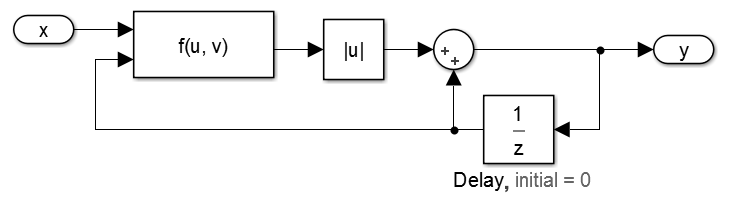
\includegraphics[width=\columnwidth]{figs/simulink.png}
%{\smaller
%\begin{verbatim}
%node filter(x : real) returns (a, b, y : real);
%let
%  a = f(x, 0.0 -> pre y);
%  b = if a >= 0.0 then a else -a;
%  y = b + (0.0 -> pre y);
%tel;
%\end{verbatim}
%}
%\vspace{-0.1in}
%\caption{Model with property $y \geq 0$, before IVC analysis}
%\label{fig:ex-before}
%\end{figure} 
\chapter{Preliminaries}
\label{sec:background}
The idea of inductive validity cores is applicable to the context of symbolic model checking using inductive proof methods. The idea is, after proving the correctness of a given property, to extract a minimal portion of the system (model) necessary for the proof of the property. In other words, we would like to determine why the property is satisfied by the system. Since this information is obtained from the inductive proofs, we call it \emph{inductive} validity core. With minimal IVCs, we are able to abstract away the part of the system irrelevant to the proof of the property. This chapter mentions some background we need for a formal description of the IVC notion.

\section{Safety Verification}

Given a state space $U$, a transition system $(I,T)$ consists of an
initial state predicate $ I : U \to \bool $ and a transition step
predicate $ T : U \times U \to \bool $.
We define the notion of
reachability for $(I, T)$ as the smallest predicate $\reach : U \to
\bool$ which satisfies the following formulas:

\begin{gather*}
  \forall u.~ I(u) \Rightarrow \reach(u) \\
  \forall u, u'.~ \reach(u) \land T(u, u') \Rightarrow \reach(u')
\end{gather*}

A safety property $P : U \to \bool$ is a state predicate. A safety
property $P$ holds on a transition system $(I, T)$ if it holds on all
reachable states, i.e., $\forall u.~ \reach(u) \Rightarrow P(u)$,
written as $\reach \Rightarrow P$ for short. When this is the case, we
write $(I, T)\vdash P$.

For an arbitrary transition system $(I, T)$, computing reachability
can be very expensive or even impossible. Thus, we need a more
effective way of checking if a safety property $P$ is satisfied by the
system. The key idea is to over-approximate reachability. If we can
find an over-approximation that implies the property, then the
property must hold. Otherwise, the approximation needs to be refined.

A good first approximation for reachability is the property itself.
That is, we can check if the following formulas hold:
\begin{gather}
  \forall u.~ I(u) \Rightarrow P(u)
  \label{eq:1-ind-base} \\
  \forall u, u'.~ P(u) \land T(u, u') \Rightarrow P(u')
  \label{eq:1-ind-step}
\end{gather}
If both formulas hold then $P$ is {\em inductive} and holds over the
system. If (\ref{eq:1-ind-base}) fails to hold, then $P$ is violated
by an initial state of the system. If (\ref{eq:1-ind-step}) fails to
hold, then $P$ is too much of an over-approximation and needs to be
refined.

One way to refine our over-approximation is to add additional lemmas
to the property of interest. For example, given another property $L :
U \to bool$ we can consider the extended property $P'(u) = P(u) \land
L(u)$, written as $P' = P \land L$ for short. If $P'$ holds on the
system, then $P$ must hold as well. The hope is that the addition of
$L$ makes formula (\ref{eq:1-ind-step}) provable because the
antecedent is more constrained. However, the consequent of
(\ref{eq:1-ind-step}) is also more constrained, so the lemma $L$ may
require additional lemmas of its own. Finding and proving these
lemmas is the means by which property directed reachability (PDR)
strengthens and proves a safety property~\cite{Een2011:PDR}.

Another way to refine our over-approximation is to use use {\em
  $k$-induction} which unrolls the property over $k$ steps of the
transition system. For example, 1-induction consists of formulas
(\ref{eq:1-ind-base}) and (\ref{eq:1-ind-step}) above, whereas
2-induction consists of the following formulas:
\begin{gather*}
\forall u.~ I(u) \Rightarrow P(u) \\
\forall u, u'.~ I(u) \land T(u, u') \Rightarrow P(u') \\
\forall u, u', u''.~ P(u) \land T(u, u') \land P(u') \land T(u',
  u'') \Rightarrow P(u'')
\end{gather*}
That is, there are two base step checks and one inductive step check.
In general, for an arbitrary $k$, $k$-induction consists of $k$
base step checks and one inductive step check as shown in
Figure~\ref{fig:k-induction} (the universal quantifiers on $u_i$ have
been elided for space). We say that a property is $k$-inductive if it
satisfies the $k$-induction constraints for the given value of $k$.
The hope is that the additional formulas in the antecedent of the
inductive step make it provable.

\begin{figure}
\begin{gather*}
I(u_0) \Rightarrow P(u_0) \\[-2pt]
%
\vdots \\[2pt]
%
I(u_0) \land T(u_0, u_1) \land \cdots \land T(u_{k-2}, u_{k-1})
\Rightarrow P(u_{k-1}) \\[2pt]
%
P(u_0) \land T(u_0, u_1) \land \cdots \land P(u_{k-1}) \land
T(u_{k-1}, u_k) \Rightarrow P(u_k)
\end{gather*}
\caption{$k$-induction formulas: $k$ base cases and one inductive
  step}
\label{fig:k-induction}
\end{figure}

In practice, inductive model checkers often use a combination of the
above techniques. Thus, a typical conclusion is of the form ``$P$ with
lemmas $L_1, \ldots, L_n$ is $k$-inductive''.


%%% Local Variables:
%%% mode: latex
%%% TeX-master: "main.tex"
%%% End

%%  LocalWords:  bool reachability JKind Lustre PDR Yices MathSAT ok
%%  LocalWords:  SMTInterpol dataflow init

%\chapter{Proposed Approach}
%\section{Related work}
\label{sec:related}

%\mike{place in related work}
%{\em Mutations and Universal Properties} It is important to note that some mutations {\em reduce} the state space of the system to be explored; in this case, any universal property (such as the safety properties in~\ref{sec:ts}) that was true of the original system must, by definition, be true of the mutated system.  For such mutations, an alternate notion of {\em vacuity coverage}
%\mike{end placement}


%Different notions of coverage have been well defined in software testing. However, in formal verification, it is very complex to define and compute this notion.
%Usually, coverage techniques in the property-based verification try to measure the quality of the specification in regard to the completeness of a set of properties.

Coverage in verification was introduced in \cite{hoskote1999coverage, katz1999have}. Hoskote et al. \cite{hoskote1999coverage} suggested a state-based metric in model checking based on FSM mutations, which are small atomic changes to the design. Then, the method for measuring coverage is to model check a given property for each mutant design.
Later in \cite{chockler_coverage_2003}, Chockler et al. provided corresponding notions of metrics used in simulation-based verification for formal verification. In fact, they improved the same idea of mutation-based coverage where each mutation is generated to check if a specific
design element is necessary for the proof of the property.
 However, the proposed algorithm is both computationally expensive and approximately linear
 in the number of mutations. Note that most of the mutation-based metrics, including \cite{kupferman_theory_2008, chockler2001practical}, are focused on finite state systems and hardware systems.

A more recent work in \cite{chockler2010coverage} performs coverage analysis through interpolation \cite{mcmillan2003interpolation}. This work is also based on design-dependent mutations \cite{chockler_coverage_2003}, where a design is considered as a net-list with nodes of types \{AND, INVERTER, REGISTER, INPUT\}.
%Each mutant design changes the type of a single node to INPUT. When property $\phi$ satisfied by the original net-list fails on the mutant design, it is said that a mutant is discovered for $\phi$, which is the same as a \emph{must} element.
%Then, the coverage metric for $\phi$ is defined as the fraction of the discovered mutants, based on which the coverage of a set of properties is measured as the fraction of mutants discovered by at least one property.
To decrease the cost of computation, coverage analysis is performed at several stages; first, all the nodes that do not appear in the resolution proof of a given property are marked as \emph{not-covered}, and the rest of the nodes are marked as \emph{unknown}. Then, for the unknown nodes, the basic mutation check is performed: if a corresponding mutant design violates the property, it will be considered as \emph{covered}. Otherwise, the algorithm tries to drive an inductive invariant to prove that the node is not covered. Finally, an interpolant-based model checking is applied to the nodes that are still unknown. This algorithm is basically the same as the \mustalg algorithm as discussed in \ref{subsec:method-disc} except that our implementation uses PDR and $k$-induction rather than interpolation.

A different approach to measure coverage involves checking whether each output signal is fully constrained by the specification \cite{das2005formal, claessen2007coverage, grosse2007estimating}. For example, in \cite{claessen2007coverage}, authors propose a design-independent coverage analysis where missing properties are identified by unconstrained output signals. Given a property list and a specific computed signal $s$ (usually drawn from the circuit outputs), if there is a trace with a point in time when $s$ is not constrained to be a single value by the set of properties and the input trace, then the property set is incomplete. Alternately, given two traces that differ only in the value of signal $s$ at a particular time step, if both traces satisfy property $P$, then $s$ is not covered by $P$.
 The work in \cite{haedicke2012guiding} refines this notion of coverage by providing a numeric score for each incompletely covered signal $s$.  Such metrics are very rigorous but can lead to overspecification: the specification must completely define the input/output function of the implementation.

A similar notion to ours was outlined in a patent~\cite{hanna2015formal}, which sketches a family of {\em proof core}-based metrics for use in hardware verification.  While the approach described by the patent is general, it is quite underspecified:
no formal description of the models, metrics, or algorithms are provided, nor in fact are any concrete metrics specified. In addition, no implementations or experimental results are provided, so it is not possible to compare their approach and ours.

 % a coverage metric that computes a numerical value to describe how much of the circuit behavior is constrained by a given set of properties. \ela{I really didn't understand the work well. I didn't read it carefully. For sure irrelevant though. we could remove this or I'll read it later}

%This methods investigates, given property $\phi$ and a specific output $s$, if there exist two traces $\sigma_{1}$ and $\sigma_{2}$ that: (1) $\sigma_{1} \vDash \phi$ and $\sigma_{2} \vDash \phi$ (2) $\forall$ signals $s' \neq s, \forall t. \sigma_{1}(t, s') = \sigma_{2}(t, s')$ (3) $\exists t. \sigma_{1}(t, s) \neq \sigma_{2}(t, s)$. This method was implemented in SMV model checker \cite{smv}.

Another technique to measure requirements completeness is to employ several surrogate models; for example, Zowghi and Gervasi~\cite{zowghi2003three} use refinement to show {\em relative completeness} with respect to a {\em domain} model, which describes the behavior of the real world, irrespective of change induced by software.  In their model, each iteration of refinement of requirements and domain models must be sufficient to prove the requirements of the previous iteration.  However, this idea has two problems: first it provides no notion of absolute completeness, and second, it requires construction of a domain model, which is often difficult and/or expensive to construct.

Outside the context of formal verification, many authors have theorised and empirically validated conceptual model completeness, which are mostly dependent on a subjective judgement \cite{drechsler2012completeness, firesmith2005your, chang2007finding,katta2013investigating, zowghi2003three, espana2009evaluating}.
%For instance, Espana et al. \cite{espana2009evaluating} also studied the granularity and completeness of specification by defining some metrics to measure completeness.

%MORE RECENT: \cite{yang2013minimal} \cite{chockler2011incremental} \cite{brillout2009mutation} \cite{bao2014coverage}: not sure if they are super relevant...
%
%MORE:
%\cite{Kupferman:2006:SCF} ? ...

%
%\cite{Whalen07:FMICS} ...



\section{Inductive Validity Cores}
\label{sec:ivc}

\newcommand{\bq}{\textsc{BaseQuery}\xspace}
\newcommand{\iq}{\textsc{IndQuery}\xspace}
\newcommand{\fq}{\textsc{FullQuery}\xspace}

\newcommand{\mink}{\textsc{MinimizeK}\xspace}
\newcommand{\reduceinv}{\textsc{ReduceInvariants}\xspace}
\newcommand{\minivc}{\textsc{MinimizeIvc}\xspace}

\newcommand{\checksat}{\textsc{CheckSat}\xspace}
\newcommand{\unsatcore}{\textsc{UnsatCore}\xspace}
\newcommand{\unsat}{\textsc{UNSAT}\xspace}
\newcommand{\sat}{\textsc{SAT}\xspace}

Given a transition system which satisfies a safety property $P$, we
want to know which parts of the system are necessary for satisfying
the safety property. One possible way of asking this is, ``What is the
most general version of this transition system that still satisfies
the property?'' The answer is disappointing. The most general system is
$I(s) = P(s)$ and $T(s, s') = P(s')$, i.e., you start in any state
satisfying the property and can transition to any state that still
satisfies the property. This answer gives no insight into the original
system because it has no connection to the original system. In this
section we introduce the notion of {\em inductive validity cores} (IVC) 
which looks at generalizing the original transition system while 
preserving a safety property.

In order to talk about generalizing a transition system, we assume the
transition relation of the system has the structure of a top-level
conjunction. This assumption gives us a structure that we can easily
manipulate as we generalize the system. Given $T(s, s') = T_1(s, s')
\land \cdots \land T_n(s, s')$ we will write $T = T_1 \land \cdots
\land T_n$ for short. By further abuse of notation we will identify
$T$ with the set of its top-level conjuncts. Thus we will write $x \in
T$ to mean that $x$ is a top-level conjuct of $T$. We will write $S
\subseteq T$ to mean that all top-level conjuncts of $S$ are top-level
conjuncts of $T$. We will write $T \setminus \{x\}$ to mean that $T$
with the top-level conjunct $x$ removed. We will use the same notation
when working with sets of invariants.

\begin{definition}{\emph{Inductive Validity Core:}}
  \label{def:ivc}
  Let $(I, T)$ be a transition system and let $P$ be a
  safety property with $(I, T)\vdash P$. We say $S \subseteq
  T$ is a {\em inductive validity core} for $(I, T)\vdash P$ iff $(I,
  S) \vdash P$. When $I$, $T$, and $P$ can be inferred from
  context we will simply say $S$ is an inductive validity core.
\end{definition}

\begin{definition}{\emph{Minimal Inductive Validity Core:}}
  \label{def:minimal-ivc}
  An inductive validity core $S$ for $(I, T)\vdash P$ is minimal iff
  there does not exist $M \subset S$ such that $M$ is an inductive validity core
  for $(I, T)\vdash P$.
\end{definition}

Note that minimal inductive validity cores are not necessarily unique.
For example, take $I = a \land b$, $T = a' \land b'$, and $P = a \lor
b$. Then both $\{a'\}$ and $\{b'\}$ are minimal inductive validity
cores for $(I, T)\vdash P$. However, inductive validity cores do have
the following monotonicity property.

\begin{lemma}
  \label{lem:ivc-monotonic}
  Let $(I, T)$ be a transition system and let $P$ be a safety property
  with $(I, T)\vdash P$. Let $S_1 \subseteq S_2 \subseteq T$. If $S_1$
  is an inductive validity core for $(I, T)\vdash P$ then $S_2$ is an
  inductive validity core for $(I, T)\vdash P$.
\end{lemma}
\begin{proof}
  From $S_1 \subseteq S_2$ we have $S_2 \Rightarrow S_1$. Thus the
  reachable states of $(I, S_2)$ are a subset of the reachable states
  of $(I, S_1)$. \qed
\end{proof}

\begin{algorithm}[t]
  \SetKwInOut{Input}{input}
  \SetKwInOut{Output}{output}
  \Input{$(I, T)\vdash P$}
  \Output{Minimal inductive validity core for $(I, T)\vdash P$}
  \BlankLine
  $S \leftarrow T$ \\
  \For{$x \in S$} {
    \If{$(I, S\setminus\{x\}) \vdash P$}{
      $S \leftarrow S\setminus \{x\}$
    }
  }
  \Return{S}
\caption{Simple algorithm for computing a minimal IVC}
\label{alg:naive}
\end{algorithm}

This lemma gives us a simple, but inefficient algorithm for computing
a minimal inductive validity core, Algorithm~\ref{alg:naive}. The
resulting set of this algorithm is obviously an inductive validity
core for $(I, T)\vdash P$. The following lemma shows that it is also
minimal.

\begin{lemma}
  The result of Algorithm~\ref{alg:naive} is a minimal inductive validity core
  for $(I, T)\vdash P$.
\end{lemma}
\begin{proof}
  Let the result be $R$. Suppose towards contradiction that $R$ is not
  minimal. Then there is an inductive validity core $M$ with $M
  \subset R$. Take $x \in R\setminus M$. Since $x \in R$ it must be
  that during the algorithm $(I, S\setminus\{x\})\vdash P$ is not true
  for some set $S$ where $R \subseteq S$. We have $M \subset R
  \subseteq S$ and $x\not\in M$, thus $M \subseteq S\setminus \{x\}$.
  Since $M$ is an inductive validity core,
  Lemma~\ref{lem:ivc-monotonic} says that $S\setminus \{x\}$ is an
  inductive validity core, and so $(I, S\setminus\{x\})\vdash P$. This
  is a contradiction, thus $R$ must be minimal.
\end{proof}

This algorithm has two problems in practice. First, checking if a
safety property holds is undecidable in general thus the algorithm may
never terminate even when the safety property is easily provable over
the original transition system. Second, this algorithm is very
inefficient since it tries to re-prove the property multiple times.

\begin{algorithm}[t]
  \SetKwInOut{Input}{input}
  \SetKwInOut{Output}{output}
  \Input{$P$ with invariants $Q$ is $k$-inductive for $(I, T)$}
  \Output{Inductive validity core for $(I, T)\vdash P$}
  \BlankLine
  $k \leftarrow \mink(T, P \land Q)$ \\
  $R \leftarrow \reduceinv_k(T, Q, P)$ \\
  \Return{$\minivc_k(I, T, R)$}\\
\caption{Efficient algorithm for computing a nearly minimal inductive validity core}
\label{alg:ivc}
\end{algorithm}

The key to a more efficient algorithm is to make better use of the
information that comes out of model checking. In addition to knowing
that $P$ holds on a system $(I, T)$, suppose we also know something
stronger: $P$ with the invariant set $Q$ is $k$-inductive for $(I,
T)$. This gives us the broad structure of a proof for $P$ which allows
us to reconstruct the proof over a modified transition system.
However, we must be careful since this proof structure may be more
than is actually needed to establish $P$. In particular, $Q$ may
contain unneeded invariants which could cause the inductive validity
core for $P \land Q$ to be larger than the inductive validity core for
$P$. Thus before computing the inductive validity core we first try to
reduce the set of invariants to be as small as possible. This
operation is expensive when $k$ is large so as a first step we
minimize $k$. This is the motivation behind
Algorithm~\ref{alg:ivc}.

\begin{figure}
\begin{align*}
  &\bq_1(I, T, P) \equiv \forall s_0.~ I(s_0) \Rightarrow P(s_0) \\
%%%
  &\bq_{k+1}(I, T, P) \equiv \bq_k(I, T, P) \land~ \\
%
  &\hspace{10pt}\left(\forall s_0, \ldots, s_k.~ I(s_0) \land T(s_0,
  s_1) \land \cdots \land T(s_{k-1}, s_k) \Rightarrow P(s_k)\right)
  \\[5pt]
%%%
  &\iq_k(T, Q, P) \equiv (\forall s_0, \ldots, s_k.~\\
%
  &\hspace{10pt} Q(s_0) \land T(s_0,
  s_1) \land \cdots \land Q(s_{k-1}) \land T(s_{k-1}, s_k) \Rightarrow
  P(s_k)) \\[5pt]
%%%
  &\fq_k(I, T, P) \equiv \\
%
  &\hspace{10pt}\bq_k(I, T, P) \land \iq_k(T, P, P)
\end{align*}
\caption{$k$-induction queries}
\label{fig:queries}
\end{figure}

To describe the details of Algorithm~\ref{alg:ivc} we define queries
for the base and inductive steps of $k$-induction
(Figure~\ref{fig:queries}). Note, in $\iq(T, Q, P)$ we separate the
assumptions made on each step, $Q$, from the property we try to show
on the last step, $P$. We use this separation when reducing the set of
invariants.

We assume that our queries are checked by an SMT solver. That is, we
assume we have a function $\checksat(F)$ which determines if $F$, an
existentially quantified formula, is satisfiable or not. In order to
efficiently manipulate our queries, we assume the ability to create
{\em activation literals} which are simply distinguished Boolean
variables. The call $\checksat(A, F)$ holds the activation literals in
$A$ true while checking $F$. When $F$ is unsatisfiable, we assume we
have a function $\unsatcore()$ which returns a minimal subset of the
activation literals such that the formula is unsatisfiable with those
activation literals held true. In practice, SMT solvers often return a
non-minimal set, but we can minimize the set via repeated calls to
\checksat.

\begin{algorithm}[t]
  $k' \leftarrow 1$ \\
  \While{$\checksat(\neg\iq_{k'}(T, P, P)) = \sat$} {
    $k' \leftarrow k' + 1$ \\
    }
  \Return{$k'$} \\
\caption{$\mink(T, P)$}
\label{alg:minimize-k}
\end{algorithm}

The function $\mink(T, P)$ is defined in
Algorithm~\ref{alg:minimize-k}. This function assumes that $P$ is
$k$-inductive for $(I, T)$. It returns the smallest $k'$ such that $P$
is $k'$-inductive for $(I, T)$. We start checking at $k' = 1$ since
smaller values of $k'$ are much quicker to check than larger ones. The
checking must eventually terminate since $P$ is $k$-inductive. We also
only check the inductive query since we know the base query will be
true for all $k' \leq k$. Although we describe each query in
Algorithm~\ref{alg:minimize-k} separately, in practice they can be
done incrementally to improve efficiency.

\begin{algorithm}[t]
  $R \leftarrow \{P\}$ \\
  Create activation literals $A = \{a_1, \ldots, a_n\}$ \\
  $C \leftarrow \{a_1 \Rightarrow Q_1, \ldots, a_n \Rightarrow Q_n\}$ \\
  \While{$true$} {
    $\checksat(A, \neg\iq_k(T, C, R))$ \\
    \If{$\unsatcore() = \emptyset$}{
      \Return{R}
    }
    \For{$a_i \in \unsatcore()$}{
      $R \leftarrow R \cup \{Q_i\}$ \\
      $C \leftarrow C \setminus \{a_i \Rightarrow Q_i\}$ \\
    }
  }
\caption{$\reduceinv_k(T, \{Q_1, \ldots, Q_n\}, P)$}
\label{alg:reduce-invariants}
\end{algorithm}

The function $\reduceinv_k(T, \{Q_1, \ldots, Q_n\}, P)$ is defined in
Algorithm~\ref{alg:reduce-invariants}. This function assumes that $P
\land Q_1 \land \cdots \land Q_n$ is $k$-inductive for $(I, T)$. It
returns a set $R \subseteq \{P, Q_1, \ldots, Q_n\}$ such that $R$ is
$k$-inductive for $(I, T)$. Like \mink, this function only checks the
inductive query since each element of $R$ is an invariant and
therefore will always pass the base query. A significant complication
for reducing invariants is that some invariants may mutually need each
other, even though none of them is needed to prove $P$. Thus in
Algorithm~\ref{alg:reduce-invariants} we find a minimal set of
invariants needed to prove $P$, then we find a minimal set of
invariants to prove those invariants, and so on. We terminate when no
more invariants are needed to prove the properties in $R$.

This iterative lemma determination does not guarantee a minimal
result. For example, we may find $P$ requires just $Q_1$, that $Q_1$
requires just $Q_2$, and that $Q_2$ does not require any other
invariants. This gives the result $\{P, Q_1, Q_2\}$, but it may be
that $Q_2$ alone is enough to prove $P$ thus the original result is
not minimal. Also note, we do not care about the result of \checksat,
only the \unsatcore that comes out of it. Since $P \land Q_1 \land
\cdots \land Q_n$ is $k$-inductive, we know the \checksat call will
always return \unsat.

\mike{I think we want to be slightly more formal in our reasoning
  about these algorithms, defining soundness (and when possible,
  minimality) lemmas for each.}
\andrew{I'm happy with the level of detail, but I'm fine if we add
  more. If you want to sketch out the outline of what you are
  thinking, I'm happy to fill in the details.}

\begin{algorithm}[t]
  Create activation literals $A = \{a_1, \ldots, a_n\}$ \\
  $T \leftarrow (a_1 \Rightarrow T_1) \land \cdots \land (a_n \Rightarrow T_n)$ \\
  $\checksat(A, \neg\fq_k(I, T, P))$ \\
  $R \leftarrow \emptyset$ \\
  \For{$a_i \in \unsatcore()$}{
    $R \leftarrow R \cup \{T_i\}$
  }
  \Return{R}
\caption{$\minivc_k(I, \{T_1, \ldots, T_n\}, P)$}
\label{alg:minimize-ivc}
\end{algorithm}

The function $\minivc_k(I, \{T_1, \ldots, T_n\}, P)$ is defined in
Algorithm~\ref{alg:minimize-ivc}. This function assumes that $P$ is
$k$-inductive for $(I, T)$. It returns a minimal inductive validity
core $R \subseteq \{T_1, \ldots, T_n\}$ such that $P$ is $k$-inductive
for $(I, R)$.

Our full inductive validity core algorithm in Algorithm~\ref{alg:ivc}
does not guarantee a minimal inductive validity core. One reason is
that \reduceinv does not guarantee a minimal set of invariants. A
larger reason is that we only consider the invariants that the
algorithm is given at the outset. It is possible that there are other
invariants which could lead to a smaller inductive validity core, but
we do not search for them. In Section~\ref{sec:exprm}, we show that in
practice our algorithm is nearly minimal and much more efficient that
the naive algorithm.

\andrew{We should find a way to clean the following argument. I'm not
  sure if it can be simplified, but perhaps we can present it better.}

In general, determining if an inductive validity core is minimal is as
hard the underlying model checking. Given a model checking question
$(I, T)\vdash^? P$ consider adding fresh varaibles $e_1$ and $e_2$ to
obtain a system with initial state predicate $I \land e_1 \land e_2$
and transition predicate $(T \land (\neg P' \Rightarrow e_1')) \land
(e_1' \Rightarrow e_2')$. This extended system has the property $P
\lor e_2$. Thus $S = \{T \land (\neg P' \Rightarrow e_1'), e_1'
\Rightarrow e_2'\}$ is an inductive validity core. Unless $P$ is a
tautology, $\{e_1' \Rightarrow e_2'\}$ will not be an inductive
validity core. The set $\{T \land (\neg P' \Rightarrow e_1')\}$ will
be an inductive validity core if and only if $(I, T)\vdash P$. Thus
decidability of minimality for inductive validity cores is as hard as
model checking.

%%% Local Variables:
%%% mode: latex
%%% TeX-master: "main.tex"
%%% End

%%  LocalWords:  Lustre iff TODO invariants Minimality BaseQuery
%%  LocalWords:  InductiveQuery FullQuery MinimizeK ReduceInvariants
%%  LocalWords:  MinimizeIVC CheckSat UnsatCore UNSAT

\section{Illustration}
\label{sec:illust}
To illustrate the \aivcalg ~algorithm we use the example presented in Section \ref{sec:example} with $P = ({\small \texttt{on\_p}})$ .
%As inspired by the MARCO algorithm in \cite{marco2016fast}, we visualize $\mathcal{P}(\mathcal{A})$ as a lattice in a Hasse diagram (Fig.~\ref{fig:lattice1}) to demonstrate the progress of the algorithm. As you can see, each level of the lattice contains sets with the same size linked to sets that are their immediate
%supersets (upper level regions) and subsets (lower level regions). Note that the power set is viewed as a Boolean formula, so each member in the lattice shows
% variable with $true$.
For better description, we view $T$ as an ordered set of its top-level conjuncts; i.e. $T = \{$ {\small \texttt{a1\_below, a2\_below, a1\_above, a2\_above, one\_below, both\_above, doi\_on, on\_p}} $\}$.
The algorithm starts with creating activation literals for each $T_i \in T$. Let the ordered set of Boolean variables $\{ a_1, \ldots , a_8 \}$ be the corresponding literals to the elements of $T$ (e.g. $\actlit ({ \small \texttt{a1\_below}}) = a_1$ and $\actlit ({\small \texttt{on\_p}}) = a_8$). Then, line 3 initializes $map$ with $\top$.

In the first iteration of the \texttt{while} loop, since $map$ is
empty, it is satisfiable, and a model for it can be any subset of
literals. So obviously, the first maximal model of $map$ contains all
the literals, which means, in line~\ref{alg:aivc:assignm}, $M = \{a_1,
\ldots, a_8\}$, and in line~\ref{alg:aivc:assigns}, $S = T$. Since $S$
is adequate for $P$, the \getivc ~module is called in
line~\ref{alg:aivc:getivc}. Suppose the returned \mivc\ by this function
is $S' = \{ { \small \texttt{a1\_below},~\texttt{one\_below},
  ~\texttt{doi\_on},~\texttt{on\_p}}\}$; this set is added to $A$ in
line~\ref{alg:aivc:addset}, and thus it comes to adding a new clause
to $map$ (line~\ref{alg:aivc:aadd}), which makes $map = (\neg a_1 \vee
\neg a_5 \vee \neg a_7 \vee \neg a_8)$. As discussed, this constraint
marks all the supersets of $S'$ as blocked and prunes them off the
search space.

For the second iteration, $map$ is still satisfiable,
so the algorithm gets to find a maximal model of it in line~\ref{alg:aivc:maxsat}. Suppose this time, the maximal model makes $M = \{a_1, \ldots, a_7\}$,
which leads to $S = T \setminus \{ {\small \texttt{on\_p}}\} $ in line~\ref{alg:aivc:assigns}.
Since $S$ is inadequate for $P$,
the algorithm jumps to line 12 updating
$map$ as $map \leftarrow map \wedge a_8$.
Adding this new clause removes all the subsets of
$T \setminus \{{\small \texttt{on\_p}}\}$
from the search space. Similarly, in the third iteration, if the maximal model of $map$
yields $M = \{a_1, \ldots, a_4, a_6, \ldots, a_8\}$, then $S = T \setminus \{ {\small \texttt{one\_below}}\} $ will be another inadequate set that makes $map$ become
$map \leftarrow map \wedge a_5$
in line~\ref{alg:aivc:iadd}.

Suppose, in the fourth iteration, the maximal model leads to $M = \{a_2, \ldots, a_8\}$ and
$S = T \setminus \{ {\small \texttt{a1\_below}}\} $ in lines~\ref{alg:aivc:assignm} and~\ref{alg:aivc:assigns}.
Since this $S$ is adequate for $P$, \getivc ~computes a new \mivc\ in line~\ref{alg:aivc:getivc}.
Let the new \mivc\ be $S' = \{ {\small \texttt{a2\_below},~\texttt{one\_below}, ~\texttt{doi\_on},~\texttt{on\_p}}\}$; after adding this set to $A$,
it is time to constrain $map$ by a new clause in line~\ref{alg:aivc:addset},
which results in $map \leftarrow map \wedge (\neg a_2 \vee \neg a_5 \vee \neg a_7 \vee \neg a_8)$.

After these iterations, $map$ is still satisfiable, and the maximal model is
 $S = T \setminus \{ { \small \texttt{a1\_below}}, { \small \texttt{a2\_below}}\}$ in line~\ref{alg:aivc:assigns}.
In this case, $S$ is inadequate, so we update $map$ as
$map \leftarrow map \wedge (a_1 \vee a_2)$ (line~\ref{alg:aivc:iadd}). After adding this new clause to $map$,
all the subsets of $T \setminus \{ { \small \texttt{a1\_below}}, {\small \texttt{a2\_below}}\}$
will be blocked. The algorithm continues similar to the forth iteration leading to $S$ (in line~\ref{alg:aivc:assigns}) and $map$ (in line~\ref{alg:aivc:iadd}) to be as
 $S = T \setminus \{ {\small  \texttt{doi\_on}}\}$ and $map \leftarrow map \wedge a_7$.

Finally, after the sixth iteration, $map$ becomes \unsat and the algorithm terminates.
Note that $MIS$es and $IVC$s may be discovered in different orders from what explained here. The order by which sets are explored is
quite dependent on the maximal model returned in line~\ref{alg:aivc:maxsat} as well as the \mivc s returned in line~\ref{alg:aivc:getivc} because there could be several distinct maximal models (\mis es) and \mivc s. For this example with a $|T| = 8$ and $|\mathcal{P}(T)| = 2^8$, a brute force approach of power set exploration needs to look into  256 cases. However, the \aivcalg ~algorithm only explored 6 cases to cover the entire power set. %Depending on the order by which \mivc s and \mis es are discovered, the total cases to explore by the algorithm may change.
% All in all, it is fair to say the \aivcalg ~algorithm is  linear in the size of $T$.
%This issue could affect the performance of the algorithm as well.



\section{Implementation}
\label{sec:impl}

We have implemented the inductive validity core algorithms in the
previous section in two tools: {\em JKind}, which performs the \ucalg
algorithm, and {\em JSupport}, which can compute either the \bfalg or
the \ucbfalg algorithm (using JKind as a subprocess). Moreover, our
implementation of \ucbfalg uses an additional feature of JKind to
store and re-use discovered invariants between separate runs. This
reduces some of the cost of attempting to re-prove a property multiple
times. These tools operate over the Lustre
language~\cite{Halbwachs91:lustre}, which we briefly illustrate below.

\subsection{Lustre and IVCs}

Lustre~\cite{Halbwachs91:lustre} is a synchronous dataflow language
used as an input language for various model checkers. The textual
models in Figures~\ref{fig:ex-before} and \ref{fig:ex-after} are
written in Lustre. We will use model in Figure~\ref{fig:ex-before} as
a running example in this section. For our purposes, a Lustre program
consists of 1) input variables, {\tt x} in the example, 2) output
variables, {\tt a}, {\tt b}, and {\tt y} in the example, and 3) an
equation for each output variable. A Lustre program runs over discrete
time steps. On each step, the input variables take on some values and
are used to compute values for the output variables on the same step.
In addition, equations may refer to the previous value of a variable
using the {\tt pre} operator. This operator is underspecified in the
initial step, so the arrow operator, {\tt ->}, is used to guard the
{\tt pre} operator. In the initial step the expression {\tt e1 -> e2}
evalutes to {\tt e1}, and it evaluates to {\tt e2} in all other steps.

We interpret a Lustre program as a model specification by considering
the behavior of the program under all possible input traces. Safety
properties over Lustre can then be expressed as Boolean expressions in
Lustre. A safety property holds if the corresponding expression is
always true for all input traces. For example, the property for
Figure~\ref{fig:ex-before} is {\tt y >= 0}, which is a valid property.

It is straightforward to translate this interpretation of Lustre into
the traditional initial and transition relations. We will show this by
continuing with the example in Figure~\ref{fig:ex-before}. First we
introduce a new Boolean variable $init$ into the state space to denote
when the system is in its initial step. Then we define,
\begin{align*}
  &I((x, a, b, y, \mathit{init})) = \mathit{init} \\
  &T((x, a, b, y, \mathit{init}), (x', a', b', y', \mathit{init'})) = \\
  &\hspace{1.5cm} (a' = f(x', \ite{init}{0}{y})) \land~ \\
  &\hspace{1.5cm} (b' = \ite{a' \geq 0}{a'}{-a'}) \land~ \\
  &\hspace{1.5cm} (y' = b' + (\ite{init}{0}{y})) \land ~\\
  &\hspace{1.5cm} \neg\mathit{init'}
\end{align*}
A safety property such as {\tt y >= 0} is translated into
$\mathit{init} \lor (y \geq 0)$. Nested uses of arrow and pre
operators are handled by introducing new output variables for nested
expressions, though such details are unimportant for our purposes.

Each equation in the Lustre program is translated into a single
top-level conjunct in the transition relation. This is very convenient
as the IVC of a Lustre property can be reported in terms of the output
variables whose equations are part of the IVC. Equivalently, the
interpretation of an IVC for a Lustre property is that any output
variable that is not part of the IVC can be turned into an input
variable, its equation thrown away, while preserving the validity of
the property.

\subsection{JKind}

JKind is an infinite-state model checker for safety properties. JKind
proves safety properties using multiple cooperative engines in
parallel including $k$-induction, property directed reachability, and
template-based lemma generation. JKind accepts Lustre programs written
over the theory of linear integer and real arithmetic. In the back-end,
JKind uses an SMT-solver such as Yices, Z3, CVC4, MathSAT, or
SMTInterpol.

JKind works on multiple properties simulatenously. When a property is
proven and IVC generation is enabled, an additional parallel engine
executes Algorithm~\ref{alg:ivc} to generate a near-minimal IVC.

JKind accepts an annotation on its input Lustre program indicating
which outputs variables to consider for IVC generation. Output
variables not mentioned in the annotation are implicitly included in
all IVCs. This allows the implementation focus on the variables
important to the user and ignore, for example, administrative
equations. This is even more important for tools which generate Lustre
as they often create many such administrative equations which simply
wire together more interesting expressions.

%
%\subsection{Experiment}
%\label{sec:experiment}

\newcommand{\takeaway}[1]{
\vspace{6pt}
\noindent\fbox{\parbox{0.975\columnwidth}{#1}}
\vspace{6pt}
}
 the overhead
in discovering all IVCs is a linear in the number of unique IVC
in the problem multiplied by the cost for finding a proof for
%\mike{What do we want to call our efficient algorithm: IVC?}

%We would like to investigate both the {\em efficiency} and {\em
%  minimality} of our three algorithms: the naive brute-force
%algorithm (\bfalg), the UNSAT core-based algorithm (\ucalg), and the
%combined UNSAT core followed by brute-force minimization algorithm
%(\ucbfalg). Efficiency is computed in terms of wall-clock time: how
%much overhead does the IVC algorithm introduce? Minimality is
%determined by the size of the IVC: cores with a smaller number of
%variables are preferred to cores with a larger number of variables.
%Finally, we are interested in the {\em diversity} of solutions: how
%often do different tools/algorithms generate different minimal IVCs?
%
%The use of \texttt{JKind} allows additional dimensions to our investigation: it supports two different inductive algorithms: $k$-induction and PDR, and a ``fastest'' mode, that runs both algorithms in parallel.  In addition, \texttt{JKind} supports multiple back-end SMT solvers including Z3~\cite{DeMoura08:z3}, Yices~\cite{Dutertre06:yices}, MathSAT~\cite{Cimatti2013:MathSAT}, and SMTInterpol~\cite{Christ2012:SMTInterpol}.  We would like to determine whether the choice of inductive algorithm affects the size of the IVC, whether different solvers are more or less efficient at producing IVCs, and whether running different solvers/algorithms leads to {\em diversity} of IVC solutions.
%
%Therefore, we investigate the following research questions:
%\begin{itemize}
%    \item \textbf{RQ1:} How expensive is it to compute inductive validity cores using the \bfalg, \ucalg, and \ucbfalg algorithms?
%    \item \textbf{RQ2:} How close to minimal are the IVC sets computed by \ucalg as opposed to the (guaranteed minimal) \ucbfalg?  How do the sizes of IVCs compare to static slices of the model?
%    \item \textbf{RQ3:} How much {\em diversity} exists in the solutions produced by different solver/induction algorithm configurations?
%\end{itemize}
%
%\subsection{Experimental Setup}
%In this study, we started from a suite of 700 Lustre models developed
%as a benchmark suite for~\cite{Hagen08:FMCAD}. We augmented this suite
%with 81 additional models from recent verification projects including
%avionics and medical devices~\cite{QFCS15:backes,hilt2013}. Most of
%the benchmark models from~\cite{Hagen08:FMCAD} are small (10kB or less,
%with 6-40 equations) and contain a range of hardware benchmarks and
%software problems involving counters. The additional models are much
%larger: around 80kB with over 300 equations. We added the new
%benchmarks to better check the scalability for the tools, especially
%with respect to the brute force algorithm.
%%
%%\mike{MORE HERE...stats on size, reasons for add'l models.}
%Each benchmark model has a single property to analyze.  For our purposes, we are only interested in models with a {\em valid} property (though it is perhaps worth noting that there is no additional computation---and thus no overhead---using the \texttt{JKind} IVC options for {\em invalid} properties).  In our benchmark set, 295 models yield counterexamples, and 10 additional models are neither provable nor yield counterexamples in our test configuration (see next paragraph for configuration information).  The benchmark suite therefore contains 476 models with valid properties, which we use as our test subjects.
%
%For each test model, we computed \ucalg in 12+1 configurations: the
%twelve configurations were the cross product of all solvers \{Z3,
%Yices, MathSAT, SMTInterpol\} and inductive algorithms
%\{$k$-induction, PDR, fastest\}, and the remaining (+1) configuration
%was an instance of \bfalg run on Yices, which is the default solver in
%\texttt{JKind}. In addition, for each of the 12 configurations, we ran an
%instance of \texttt{JKind} without IVC to examine overhead. The experiments
%were run on an Intel(R) i5-2430M, 2.40GHz, 4GB memory machine, with a
%1 hour timeout for each analysis on any model. The data gathered for
%each configuration of each model included the time required to check
%the model without IVC, with IVC, and also the set of elements in the
%computed IVC.\footnote{The benchmarks, all raw experimental results,
%  and computed data are available on \cite{expr}.}
%
%Note that not all analysis problems were solvable with all algorithms: for all solvers, $k$-induction (without IVC) was unable to solve 172 of the examples.  When comparing minimality of different solving algorithms, we only considered cases where both algorithms provided a solution (as will be discussed in more detail in Section~\ref{sec:minimality}).
%
%\iffalse
%\begin{itemize}
%    \item an algorithm to compute a truly minimal set of support, i.e. \texttt{JSupport}.
%    \item given a LUS model, a static crawler which automatically marks all equations of a node in the initial support set of a property.
%    \item some trackers that measure the verification time with/ without support computation.
%   % \item some minor changes in the XML writers.
%\end{itemize}
%
%\mike{My thoughts on this section: mostly, it needs more structure: more information on the properties of the models: size, provenance, etc., a broken out subsection on the description of the experimental setup, etc}
%
%\mike{I think we want to split out the results in another top-level section}
%
%Experiment:
%\begin{itemize}
%    \item (Overview) describe research questions and goals.
%    \item Experimental setup: tell me about the models: how many, how big are they?  Then, tell me about the experiment: the tool configurations, the machine used for test.
%    \item Data generation: Describe what you measured for each model analysis.
%\end{itemize}
%\fi
%
%
%%%  LocalWords:  minimality ive UNSAT IVC Minimality IVCs PDR Yices
%%%  LocalWords:  MathSAT SMTInterpol RQ JSupport


\chapter{Applications}
\label{sec:apps}
As described in Section \ref{ch:intro}, IVCs can facilitate several engineering tasks in different phases of a system development process. This chapter explains some of the IVC applications we have explored.
\iffalse
Safety-critical systems, like an airborne software, must undergo a rigorous software development process usually governed by particular standards, such as DO-178C for Software Considerations in Airborne Systems and Equipment Certification \cite{DO178C} and DO-333 for Formal Methods Supplement to DO-178C and DO-278A \cite{DO333}.
DO-178C proposes a rigorous software development process that starts with an abstract requirements artifact that is iteratively refined into a software designs, source code, and finally, object code, and a set of {\em objectives} that should be met by critical avionics software.  Two of the key tenets of this process are traceability and adequacy; that is, each refinement of an artifact must be traceable to the artifact if was derived from. Further, each refinement must be shown not to introduce functionality not present in the artifact from which it was derived (adequacy). For example, DO-178C objectives A-3.6 (traceability of high-level requirements to system requirements) and A-4.6 (traceability of software design to high-level requirements) specifically require applicants to demonstrate bi-directional traceability.

DO178C currently uses a variety of metrics to determine adequacy of requirements, but much of the effort involves code-level testing.  Test suites are derived from requirements and used to test the software and measured using different structural coverage test metrics.  If code-level test suites do not achieve full coverage, then an analysis is performed to determine whether there are missing requirements and test cases.  The kind of structural coverage required (e.g., statement, branch, MCDC) for adequate testing is driven by the criticality of the software in question.

The utility of the IVCs are being evaluated by Rockwell Collins on a pilot project for both traceability and adequacy checking \cite{lucas17}. Previously, bi-directional traceability between artifacts involved tedious manual peer review to determine that requirements were adequate and that additional functionality was not introduced in the implementation model. IVCs offer automation to satisfy the DO178C objectives related to traceability and adequacy, which is a very important use in providing certifications. This section describes how IVCs can be employed for traceability and adequacy checking.
\fi

\section{Automatic Proof-Based Traceability}


\section{Preliminaries}
\label{sec:background}
\newcommand{\satisfies}{\vdash_{\!\!s}}
\newcommand{\nsatisfies}{\nvdash_{\!\!s}}
\newcommand{\bool}[0]{\mathit{bool}}
\newcommand{\reach}[0]{\mathit{R}}
\newcommand{\ite}[3]{\mathit{if}\ {#1}\ \mathit{then}\ {#2}\ \mathit{else}\ {#3}}
\newcommand{\nondetcov}{\text{\sc Nondet-Cov}}
\newcommand{\mutcov}{\text{\sc Mutant-Cov}}

\subsection{Models, Requirements, and Provability}

We define \emph{provability} of a requirement with respect to a model independent of a particular proof system.  We define the implementation model as a set of formulas $\Gamma$  and the set of requirements $\Delta$.
Then given $\Gamma' \subseteq \Gamma$ and $\delta \in \Delta$, we use the notation $\Gamma' \vdash \delta$ to mean that $\delta$ is \emph{provable} given the set $\Gamma'$.  We assume that the provability relation $\vdash$ is monotonic on the subset relation over $\Gamma$, that is, if $\Gamma'' \subseteq \Gamma' \subseteq \Gamma$ and $\Gamma'' \vdash \delta$, then $\Gamma' \vdash \delta$.  The monotonicity of the satisfaction relation means that, unless {\em all} elements of the implementation $\Gamma$ are required for a proof, there are multiple implementation sets $\Gamma'' \subset \Gamma' \subset \ldots \subset \Gamma$ that can satisfy a given requirement $\delta$.  In an abuse of notation, we write $\Gamma' \vdash \Delta$ to mean the conjunction of all requirements in $\Delta$: $\Gamma' \vdash \bigwedge \Delta$.

\subsubsection{Example: Transition Systems}
\label{sec:ts}
We can straightforwardly instantiate our abstract model over a transition system for proving safety properties.  Given a state space $S$, a transition system $(I,T)$ consists of an initial state predicate $I : S \to \bool$ and a transition step predicate $T : S \times S \to \bool$. We define the notion of reachability for $(I, T)$ as the smallest predicate $\reach : S \to \bool$ which satisfies the following formulas:
\begin{gather*}
  \forall s.~ I(s) \Rightarrow \reach(s) \\
  \forall s, s'.~ \reach(s) \land T(s, s') \Rightarrow \reach(s')
\end{gather*}
A safety property $P : S \to \bool$ is a state predicate. A safety property $P$ holds on a transition system $(I, T)$ if it holds on all reachable states, i.e., $\forall s.~ \reach(s) \Rightarrow P(s)$, written as $\reach \Rightarrow P$ for short. When this is the case, we write $(I, T)\vdash_{T} P$, for provability within the transition system.  We assume the transition relation of the system has the structure of a top-level conjunction. This assumption gives us a structure that we can easily manipulate. Given $T(s, s') = T_1(s, s') \land \cdots \land T_n(s, s')$ we will write $T = T_1 \land \cdots \land T_n$ for short. By further abuse of notation we will identify $T$ with the set of its top-level conjuncts. Thus we will write $x \in T$ to mean that $x$ is a top-level conjunct of $T$; or, equivalently, $\Gamma = \{T_1, T_2, \ldots, T_n\}$ and $\Delta = \{P\}$ in our abstract model.

Such a transition system can easily encode our example model in Section~\ref{sec:example}.  We assume each equation defines a conjunct within the transition system which we will denote by the variable assigned, so $\Gamma = \{$ {\small \texttt{a1\_below, a2\_below, a1\_above, a2\_above, below, above\_hyst}} $\}$.
%\footnote{In the example in Section \ref{sec:example}, $\Gamma = \{{\tt P}, {\tt x}, {\tt c1}, {\tt c2}, {\tt c3}, {\tt r1}, {\tt r2}\}$ and $\Delta = \{{\tt P}\}$.}

%Such transition systems can represent either finite or infinite state systems, depending on the state space $S$.

%We will write $S \subseteq T$ to mean that all top-level conjuncts of $S$ are top-level conjuncts of $T$. We will write $T \setminus \{x\}$ to mean $T$ with the top-level conjunct $x$ removed.


%\paragraph{Applying Provability to Transition Relations and Safety Properties}

%\mike{To do: add a few paragraphs on instantiating the formal model for transition systems and model checking (a la IVCs), then further elaborate it for Netlists (a la Chockler and Kroening).}

%\mike{We could cover tableau methods here, but these are overly restrictive}

\subsection{Requirements Coverage and Mutations}
The goal of a coverage metric is usually to assign a numeric score that describes how well requirements cover the design.  The majority of the work in requirements coverage metrics has focused on {\em mutations}, which are ``atomic'' changes to the design, where the set of possible mutations depends on the notation that is used.  A mutant is ``killed'' if one of the requirements that is satisfied by the original design is violated by the mutated design~\cite{chockler_coverage_2003,chockler2001practical,chockler2010coverage,Kupferman:2006:SCF,kupferman_theory_2008}.  There are Many different kinds of mutations that have been proposed, primarily focused on checking sequential bit-level hardware designs.  For these designs, {\em State-based} mutations flip the value of one of the bits in the state.  There are several variations depending on whether the flip is performed on a single state within a Kripke structure~\cite{hoskote1999coverage}, or in the description of the signal in the transition relation of the circuit~\cite{chockler2001practical}.  {\em Logic-based} mutations fix the value of a bit to constant zero or one, and can be used to determine whether requirements can find stuck-at faults.  {\em Syntactic} mutations~\cite{chockler_coverage_2003} remove states in a control flow graph representation of hardware.  Similarly, for software, it is possible to apply any of the ``standard'' source code mutation operators used for software testing~\cite{Andrews06:mutation} towards requirements coverage analysis.  Some examples of software mutations are: 
\begin{enumerate}
    \item Replace an integer constant C by one of $\{0, 1, -1, C + 1, C - 1\}$.
    \item Replace an arithmetic, relational, logical, bitwise logical, increment/decrement, or arithmetic-assignment operator by another operator from the same class.
    \item Negate the decision in an if or while statement
    \item Delete a statement
\end{enumerate}


For our abstract model, we assume each element $\gamma \in \Gamma$ has a set of possible mutations associated with it.  Depending on the modeling formalism used, this may be the value of a gate or signal or an expression within a statement in a program.  We will further assume the existence of a mutation function $f_{m}$ that, given a model element, will return a finite set of mutations for that element.  We can then define the set of mutant models $M$ as follows:
\[
    M = \{ \gamma \in \Gamma, m \in f_{m}(\gamma)\ |\ \Gamma - \{\gamma\} \cup \{m\} \}
\]

\noindent and then define the mutation score for a set of requirements $\Gamma$ in the standard way:

\begin{definition} {\emph{Generalized mutation coverage.} } \\
\[
   \mutcov = \frac{ | \{m \in M(\Gamma)~|~ m \nvdash \Delta\} |}{|M(\Gamma)|}
\]
\end{definition}

%\mike{Do we want these parameterized?  We could just assume Gamma and Delta}

In our example in Figure~\ref{fig:asw}, applying the software mutations from~\cite{Andrews06:mutation} would involve manipulating the constants used in the definitions of \texttt{a1\_below, a2\_below, a1\_above, a2\_above}, swapping 'or' and 'and' in the definition of \texttt{below, above\_hyst}, or negating the conditions in the if/then/else statements.  Even for this small model, note that there are a large number of possible mutations: 57 given the set defined above, and that this number increases rapidly with the size of the program and the chosen set of mutations.


%\mike{Illustrate on running example here.}

Of particular interest is the mutation that replaces a computed variable ({\em signal} in hardware) with a ``fresh'' input; this mutation is called a {\em nondeterminism mutation} with a coverage metric called (\nondetcov)~\cite{chockler2010coverage} and is discussed in~\cite{Kupferman:2006:SCF,kupferman_theory_2008,chockler2010coverage}.  If we use an equational transition system to assign the variables, then performing \nondetcov\ coverage an isomorphic operation to removing the defining equation from the set $\Gamma$ and checking whether provability is preserved.  In this case, we can dispense with the set $M$ and compute a mutation score much more simply:

\begin{definition} {\emph{Nondeterministic coverage.} }
\[
   \nondetcov = \frac{ | \{\gamma \in \Gamma~|~ \Gamma - \{\gamma\} \nvdash \Delta\} |}{|\Gamma|}
\]
\end{definition}

\noindent In one sense, the nondeterminism mutation is the {\em strongest} mutation because it introduces the most additional behaviors into the model, that is, any execution sequence constructed by modifying the assigning equation is also an execution sequence for a nondeterministic mutation.  Equivalently, given a set of universal properties, it is the easiest mutation to ``kill''.  For our example in Figure~\ref{fig:asw}, this mutation would lead to 10 mutations, one for each equation in the model.

%\mike{Illustrate on running example here}

\iffalse
\subsection{Requirements Coverage and Structural Testing}
\mike{not sure we need this...if so, we need to accurately characterize test obligations as a function from elements in $\Gamma$}
In {\em black-box} testing, one is interested in creating a suite of tests from requirements that adequately exercise the behavior
of a software system without regard to the internal structure of the implementation.  This is the preferred style of testing in
safety-critical domains and is advocated by standards such as DO-178B~\cite{RTCA:DO-178B}.  The adequacy of such test suites are usually inferred by examining different coverage metrics on an executable artifact, either source code~\cite{Bezier90:TestingBook,MCDCPaper} or software models~\cite{Ammann99:SpecBasedCoverageMetric,Sanjai03:dissertation}.  If the tests are not sufficient to cover the structure of the code, then either additional tests are derived from existing requirements, or (often) additional requirements are created to describe the additional functionality that is not covered by any tests.

Common metrics used for test coverage measurement are {\em statement}, {\em decision}, and {\em modified condition/decision coverage (MCDC)}.  In this section, we use the rigorous MCDC metric to measure coverage.  \mike{Define MCDC}.

It is straightforward to define coverage in a way that is parametric to the particular test metric that is used.  Given a set $\Theta$ of all possible tests and $\Phi$ the set of all {\em test obligations} induced by the test metric over the model, we define three functions.  The first, $R_m : \Delta \rightarrow 2^\Theta$, defines the set of tests furnished for each requirement.  The second, $E_m : \Gamma \rightarrow 2^\Phi$ defines the test obligations associated with each model element.  The third, $T_m : \Theta \rightarrow 2^\Phi$, defines the obligations that are covered by the test.  Then coverage can be defined as: $$\frac{|\bigcup_{t \in T} T_m (t)|}{|\Phi|}$$.


%Formally, irrespective of the metric used, given $T$ the set of all tests, and the user furnishes test cases associated with each requirement: . Coverage for a given test is measured using a function that maps tests to model elements  as follows \cite{chelenski1994oapplicability, schuler_assessing_2011, murugesan2015we}: $$\frac{|\bigcup_{t \in T} T_m (t, \Gamma)|}{|\Gamma|}$$

%
%\mike{revise}
%

A common problem with this metric is masking:
the effect of a change in a variable cannot be observed in the output. To illustrate, consider the example in Fig. \ref{fig:ex}; suppose we are provided with
test suite \{\{{\tt in1} = \emph{true}, {\tt in2} = \emph{false}\},
\{{\tt in1} = \emph{false}, {\tt in2} = \emph{false}\}\}. The change in the value of
{\tt in1} is masked by {\tt c1}. This problem causes the coverage method reports something covered
while it actually does not affect the output at all.



%\noindent In the following sections, we will examine other possible scoring mechanisms based on minimal provability, and contrast them against testing and vacuity-based metrics.

%\begin{figure}[htb]
%\begin{center}
%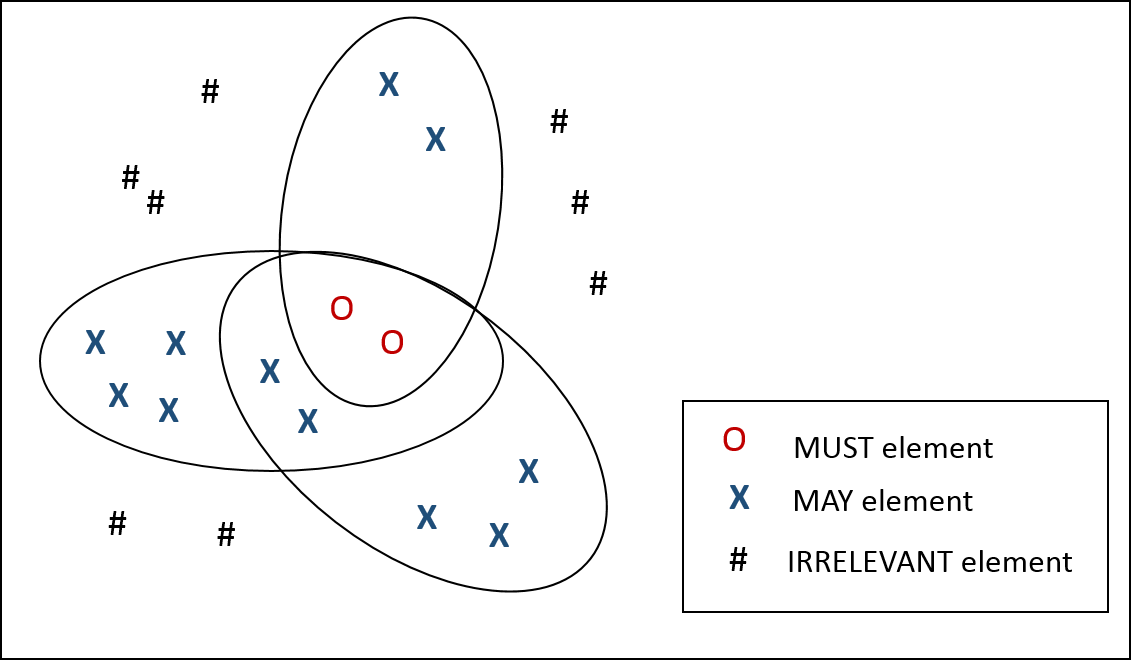
\includegraphics[width=\columnwidth]{figs/may_must.png}
%\caption{A visual example of partitioning the implementation model}\label{fig:maymust}
%\end{center}
%\end{figure}

\iffalse
In light of this intuition, we define existing coverage notions in the literature, which are based on the idea of \emph{mutation}. Then, later, we explore some novel notions of coverage based on the idea of support sets.  More formally, mutation, denoted by $f_m$, is a relation that maps $\Gamma$ to set $S \subset \Gamma$ (written as $f_m (S)$). The range of $f_m$ for $\Gamma$ is denoted by $M$.

In general, requirements completeness can be defined with regard to the notion of \emph{coverage}. In fact, the way that coverage is formalized plays a key part in the strength/ effectiveness of a method for the assessment of completeness. Requirements completeness can be judged on a fraction called \emph{coverage score}, the closer to 1 the score is, the more complete the specification is.

\begin{definition}{\emph{Coverage:}}
  \label{def:coverage}
   Any notion of coverage can be formalized as a function $\psi$ such that,
   $\forall r \in \Delta, \varphi \in \Gamma$, if $\varphi$ is covered by $r$ then $\psi (r, \varphi) = true$, denoted by $\psi (r) \preccurlyeq \varphi$, otherwise  $\psi (r, \varphi) = false$, denoted by $\psi (r) \nprec \varphi$.
\end{definition}

\begin{definition} {\emph{Coverage based on single mutation \cite{chockler2010coverage, chockler_coverage_2003}:}}
  \label{def:coverage1}
   $\forall r \in \Delta$,
   $\varphi \in \Gamma$,
   $\psi (r) \preccurlyeq \varphi$
   iff $\Gamma \vdash r$ and
   $f_m (\Gamma \setminus \{ \varphi \}) \nvdash r$. Otherwise, $\psi (r) \nprec \varphi$.
\end{definition}

For the sake of simplicity, we refer to the coverage function
formalized in Definition \ref{def:coverage1} as $\psi_{sm}$.
Back to our example, $\psi_{sm}$ only considers {\tt P} and {\tt c3} as covered in the model shown in Fig. \ref{fig:ex}.

Using $\psi_{sm}$, the coverage score of specification $r$ is computed by $$\frac{\sum_{\varphi \in \Gamma} f_m (\Gamma \setminus \{ \varphi \}) \nvdash r}{|\Gamma|}$$
Usually, a mutation is an atomic change to the design whose effect is not masked by other modifications, which means simultaneous mutations may result in masking the changes. However,
it is possible to define the coverage notion with regard to all possible mutations, although it would be also very expensive and impractical \cite{chockler2001practical}. \ela{Mike, is the citation correct?}.
For a coverage function based on all mutations, the coverage score is calculated by
$$ \frac{\sum_{S \in M} f_m (S) \nvdash r}{|\Gamma| |M|}$$
\fi
\fi





\section{Coverage Analysis and Requirements Completeness}

For critical systems, it has been argued that formal methods
%, involving formalized requirements and proofs of implementation correctness,
should be applied to gain higher assurance than is possible with testing~\cite{Miller10:CACM,Rushby09:SEFM,Hardin09:Security}.  For these approaches, testing may still be performed, but the verification effort is primarily focused on performing proofs.  Unfortunately, proof-based approaches tend not to answer the question as to whether implementations have {\em additional functionality} that is not covered by requirements.  %Testing, despite its faults, can measure {\em structural coverage} to find untested functionality and can find some errors by {\em serendipity}, in which problems not directly related to the requirement under test are exposed.  Therefore, in formal verification approaches, it is even more important that requirements be complete.
%
Thus, we are interested in notions of {\em coverage}: determining how well the requirements characterize the implementation model.
The goal of a {\em coverage metric} is usually to assign a numeric score that describes how well properties cover the design.

Relatively recently, techniques have been devised for analyzing completeness of requirements against formal implementation models, specified as transition systems or Kripke structures \cite{chockler2001practical,das2005formal, claessen2007coverage, grosse2007estimating,chockler_coverage_2003,chockler2010coverage,
Kupferman:2006:SCF,kupferman_theory_2008}.  These models are agnostic to the abstraction level of the implementation: implementations can be lower-level requirements, software architectures, or concrete implementations of system behavior.  The mechanism used is based on {\em mutation} and {\em proof}: is it possible to prove that the requirements still hold of the system after mutating the model in some way?  If so, then the requirements are incomplete with respect to that model element.


\iffalse
Mutations are ``atomic'' changes to the design, where the set of possible mutations depends on the notation that is used.  A mutant is ``killed'' if one of the properties that is satisfied by the original design is violated by the mutated design~\cite{chockler_coverage_2003,chockler2001practical,chockler2010coverage,Kupferman:2006:SCF,kupferman_theory_2008}.  There are many different kinds of mutations that have been proposed, primarily focused on checking sequential bit-level hardware designs.
For these designs, {\em State-based} mutations flip the value of one of the bits in the state.  There are several variations depending on whether the flip is performed on a single state within a Kripke structure~\cite{hoskote1999coverage}, or in the description of the signal in the transition relation of the circuit~\cite{chockler2001practical}.  {\em Logic-based} mutations fix the value of a bit to constant zero or one, and can be used to determine whether properties can find stuck-at faults.  {\em Syntactic} mutations~\cite{chockler_coverage_2003} remove states in a control flow graph representation of hardware.
Similarly, for software, it is possible to apply any of the ``standard'' source code mutation operators used for software testing~\cite{Andrews06:mutation} towards requirements coverage analysis.
Some examples of software mutations are \cite{Budd:1980}:
\begin{enumerate}
    \item Replace an integer constant $C$ by one of $\{0, 1, -1, C + 1, C - 1\}$,
    \item Replace an arithmetic, relational, logical, bitwise logical, increment/decrement, or arithmetic-assignment operator by another operator from the same class,
    \item Negate the decision in an \texttt{if} or \texttt{while} statement,
    \item Delete a statement.
\end{enumerate}

We assume each element $T_i \in T$ has a set of possible mutations associated with it.  Depending on the modeling formalism used, this may be the value of a gate or signal or an expression within a statement in a program.  We will further assume the existence of a mutation function $f_{m}$ that, given a model element, will return a finite set of mutations for that element.  We can then define the set of mutant models $M$ as follows:
\[
    M = \{ (T \setminus \{T_i\}) \cup \{m\} \ |\ T_i \in T, m \in f_{m}(T_i) \}
\]
\noindent and then define the mutation score for property $P$ in the standard way:
\begin{definition} {\emph{Generalized mutation coverage.} } \\
\[
   \mutcov = \frac{ | \{m~|~ m \in M~\land~(I, m) \nvdash P\} |}{|M|}
\]
\end{definition}

\noindent Note that without loss of generality, we consider a single property $P$, which can be viewed as the conjunction of all the properties of the model.

The state of the art of mutation-based coverage can be found in Chockler \textit{et al.} \cite{chockler2010coverage}, where a design is considered as a net-list with nodes of types {\small \texttt{\{AND, INVERTER, REGISTER, INPUT\}}}.
Each mutant design changes the type of a single node to {\small \texttt{INPUT}}. When property $\phi$ satisfied by the original net-list fails on the mutant design, it is said that a mutant is discovered for $\phi$. Then, the coverage metric for $\phi$ is defined as the fraction of the discovered mutants, based on which the coverage of a set of properties is measured as the fraction of mutants discovered by at least one property.
To decrease the cost of computation, coverage analysis is performed at several stages; first, all the nodes that do not appear in the resolution proof of a given property are marked as \emph{not-covered}, and the rest of the nodes are marked as \emph{unknown}. Then, for the unknown nodes, the basic mutation check is performed: if a corresponding mutant design violates the property, it will be considered as \emph{covered}.
\fi

Unfortunately, previous metrics based on mutation are expensive to compute, as they involve running many different verification efforts against mutant models.  For example, given a mutant generator developed for testing Lustre programs~\cite{jkind}, the 50 largest models in the benchmark suite each had more than 30,000 mutants.  While it is possible to approximate mutation coverage scores using sampling~\cite{Zhang13:sampling}, samples still often require 5\% or more of the possible mutants.  One can also restrict the set of possible mutations, but this runs the risk of biasing the program to miss certain kinds of faults.

Thus, we propose a new family of metrics for measuring property completeness based on proofs and \mivc s rather than mutation.  These metrics are based on the notions of \mivc s and MAY and MUST elements introduced in the previous section.  The metrics have benefits in that they are cheaper to compute than previous metrics (especially the \mivc\ metric) and have a formal basis provided by proofs.

For the purposes of this discussion of coverage, without loss of generality, we assume that the analysis is performed over a single property $P$ (which may represent the conjunction of all of the properties for the model).

%they can {\em underapproximate} the portion of the model necessary for proof
%can {\em underapproximate} which portions of an implementation model are necessary to produce a proof.
%completeness metrics can {\em underapproximate} which portions of a program are necessary to fulfill the requirements.  That is, if we construct a model consisting of only the required model elements as determined by the analysis, it is often no longer possible to prove the requirement.  Thus the feedback provided to the developer may be somewhat misleading.  In addition, the mutation-based analyses tend to be very computationally expensive.  For example, for model checkers, state of the art techniques have runtimes of (in the best case) several times more than is required for proof~\cite{chockler2010coverage}.


%\footnote{Section~\ref{sec:impl} describes how these proofs are discovered in practice.}
%\subsection{Coverage and Minimal Proofs}
%Alternatively, we can consider using the proofs themselves as a mechanism for determining adequacy of requirements.

\begin{definition} {\emph{IVC coverage (\ivccov):}} \\
\label{def:coverage-justi}
Given $S \in \aivc(P)$, $T_i$ is covered by $P$ via $S$ \emph{iff} $T_i \in S$.
\end{definition}

%We call Definition \ref{def:coverage-justi} a \emph{proof-preserving} metric because, with a set of the model elements marked as covered by \ivccov ,
%$P$ is provable.  %Other notions, as will be discussed,
%may yield subsets of the model that are insufficient to
%reconstruct the proof of the property.
%\footnote{\noindent ~Throughout the paper, when a coverage metric is justifiable, like \ivccov, we say that it preserves provability of the property.}
%Thus, the coverage score for \ivccov\ is often higher than the score for \nondetcov.
The coverage score for \ivccov\ can be calculated with: $$\frac{|S|}{|T|}$$  where $|T|$ is the number of conjuncts in $T$.
%Note that because minimal proofs are not unique, there are several possible coverage scores.
Because $P$ may have multiple \mivc s,
  \ivccov\ metric can lead to various scores that belong to the following set:
\[
\left\{~\frac{ |S|}{|T|}~\bigg|~S \in AIVC(P)~\right\}
\]

\noindent Note that if an \mivc ~contains all model elements (i.e., the model is {\em completely covered}), then there is only one possible \mivc , so in this case there is no diversity of scores. On the other hand, a set of states and signals can be considered covered or not covered depending on a particular \mivc\ we consider for coverage evaluation. To address this issue, we introduce additional coverage metrics using the notions of \may\ and \must.

%Since the primary goal of
% this paper has been to provide a complementary coverage notion in
%  formal verification, it is worth exploring other possible notions based on the idea of provability and $\aivc$, which is beneficial, as with testing, because if a coverage notion is an over-approximation, when the coverage
% is high, it does not necessarily mean the quality of
% the specification (or test suite) is high, or when it is an under-approximation, a low coverage score does not always mean the specification is of poor quality.

\begin{definition} {\emph{(\maycov):}}
  \label{def:comp-1}
 $T_i \in T$ is covered by $P$ \emph{iff} $T_i \in \maycov (P)$, where
   $\maycov (P) = \{T_i ~|~ \exists S \in \aivc(P)~.~T_i \in S \}$.
\end{definition}

\begin{definition} {\emph{(\mustcov):}}
  \label{def:mustcov}
 $T_i \in T$ is covered by $P$ \emph{iff} $T_i \in \mustcov (P)$, where
   $\mustcov (P) = \{T_i ~|~ \forall S \in \aivc(P)~.~T_i \in S \}$.
\end{definition}

The $\maycov$ notion considers a model element covered if it is found in any \mivc ; thus it is a weaker notion of coverage for models with multiple \mivc s, but has the benefit of being uniquely defined.  \mustcov\ takes the opposite view, considering a model element as covered only if it affects all the proofs of $P$.

\iffalse
Algorithm \ref{alg:must} is also an efficient way of computing the \emph{must} set of a given property using \ucalg. A different algorithm for computing $\must (P)$ is to first compute $\aivc (P)$ and then take the intersection of all sets in $\aivc (P)$.


\begin{algorithm}
  \SetKwInOut{Input}{input}
  \SetKwInOut{Output}{output}
  \Input{$(I, T) \vdash P$}
  \Output{Must set for $(I, T) \vdash P$}
  \BlankLine
  $S \leftarrow \ucalg((I, T) \vdash P)$ \\
  $M \leftarrow \varnothing$ \\
  \For{$x \in S$} {
    \If{$(I, T\setminus\{x\}) \nvdash P$}{
      $M = M \cup \{x\}$
    }
  }
  \Return{M}
\caption{\mustalg: an algorithm to compute $\must(P)$ for a given $P$}
\label{alg:must}
\end{algorithm}
\fi

\iffalse
It is still possible to build more relaxed coverage metrics in which coverage
is captured by looking at individual properties, rather than their conjunction.
%for example, in the definition of \ivccov , it is wise to look at $P$ as
%the conjunction of all properties. However,
We can, for example, describe a metric in which any element used by an \mivc ~for any property is considered covered.
%with this view,
%elements around IVCs that do not have common \emph{must}
%elements with others will be treated as uncovered while they are at least covered by one
% IVC of an individual property in the specification.
%
The next definition, \allcov, formalizes this notion.
\begin{definition} {\emph{(\allcov):}}
  \label{def:comp-2}
     Given a set of properties $\Delta$ over $T$, $T_i \in T$ is covered
   \emph{iff} $T_i \in \allcov (T)$, where
   $\allcov (T) = \{T_i ~|~ \exists P \in \Delta ,~ S \in \aivc(P).~T_i \in S \}$.
\end{definition}

\fi

\iffalse
Based on the categorization of elements, we will state a relationship about \mivc s in order to compare different proof-based metrics proposed earlier.

\begin{lemma}
  \label{lem:must-not-enough}
  If $\may(P) \neq \varnothing$, then $P$ is not provable by $\must(P)$.
\end{lemma}
\begin{proof}
  $\may(P) \neq \varnothing \Rightarrow  \exists T_i \in \may(P).$
$T_i \in \bigcup \aivc(P) \wedge T_i \notin \must(P)$,
which implies $\exists S \in \aivc(P).~ T_i \in S$.
Considering the fact that $S$ is minimal and
$\must(P) \subset S$ (since $T_i \in S \wedge T_i \notin \must(P)$),
 $\nexists S' \subset S.~ (I,S') \vdash P$,  which means $(I, \must(P)) \nvdash P$.
\end{proof}
\vspace{2mm}

\fi

%\begin{lemma}
%    \label{lem:must-mustcov}
%    $T_i \in \must(P) \Leftrightarrow T_i \in \mustcov(P)$
%\end{lemma}
%\begin{proof}
%Immediate from the definition of $\must$ and \mustcov.
%\end{proof}

\iffalse
Now we focus on the relationship between non-deterministic mutation-based coverage and proof-based metrics. In Chockler et. al.
~\cite{chockler2010coverage},
each mutant design changes the type of a single node to an input node .
Given a suitable encoding of the netlist, assigning a ``fresh'' input is an isomorphic operation to simply removing a $T_i$ from $T$. The mapping is as follows: the net-list becomes a conjunction
of equations, where each vertex becomes a variable $v_i \in U$, and where each non-input vertex becomes an assignment equation $T_i \in T$.
For example, given an AND-vertex $v_i$ with three input edges from other vertexes $\{v_a, v_b, v_c\}$, we would define an equation $T_i \in T$ of the form $(v_i = (v_a \wedge v_b \wedge v_c))$.
%
%As the variable is no longer constrained by a defining equation, it is effectively an %input.

Given this encoding, we can reframe the non-deterministic coverage proposed in \cite{chockler2010coverage} as follows:

\begin{definition} {\emph{Nondeterministic coverage (alternate specification) (\nondetcovalt) ~\cite{chockler2010coverage}.} }
\label{def:non-det-2}
$T_i \in T$ is covered by property $P$ \emph{iff} $T_i \in \nondetcovalt (P)$, where
$\nondetcovalt (P) = \{T_i~|~ (I, T) \vdash P \wedge (I, T \setminus \{T_i\}) \nvdash P\}$.
\end{definition}
\noindent Given this definition, it becomes straightforward to define some additional properties.

\begin{lemma}
  \label{lem:must-coverage}
$T_i \in \nondetcovalt (P) \Leftrightarrow T_i \in \mustcov(P)$.
\end{lemma}
\begin{proof}
$T_i \in \nondetcovalt (P)$ means that $(I, T \setminus \{ T_i \}) \nvdash P$ then
%$T_i$ is necessary to prove $P$,  which means
$\forall S \subset T .~ T_i \notin S \Rightarrow (I, S) \nvdash P$.
Therefore, since $(I, T) \vdash P$, $T_i \in \bigcap \aivc(P)$, which means  $T_i \in \must(P)$.
On the other hand, let $T_i \in \must(P)$; then $\forall S \in \aivc(P).~ T_i \in S$.
By definition, any proof of $P$ is a superset of some minimal IVC in $\aivc(P)$.
Thus, any subset $S$ of $T$ leading to proof contains $T_i$.
Therefore, $T \setminus \{ T_i \}$ does not lead to a proof.

\end{proof}
\vspace{2mm}

In light of Lemma \ref{lem:must-coverage}, the \nondetcovalt\ coverage score of specification $P$ can be also calculated by
$$\frac{|\must(P)|}{|T|}$$
%Therefore, for set of properties $\Delta$, the coverage score is computed by $$\frac{|\must(\Pi)|}{|T|},\quad  \Pi= \bigwedge_{i} {P_i \in \Delta}$$


%\mike{after all metrics presented, contrast them on the example.  Introduce the properties HERE and then discuss the coverage sets}
%
%\mike{Then, you can talk about justification, etc.}
\begin{corollary}
\label{cor:must-not-provable}
\nondetcovalt\ is not proof-preserving.
\end{corollary}
\begin{proof}
Immediate from Lemma \ref{lem:must-not-enough} and Lemma \ref{lem:must-coverage}
\end{proof}
\vspace{2mm}
\begin{corollary}
\label{cor:ivc-provable}
\ivccov\ is proof-preserving.
\end{corollary}
\begin{proof}
Immediate from Definition~\ref{def:minimal-ivc} and Definition \ref{def:coverage-justi}
\end{proof}
\vspace{2mm}

%It should be pointed out that \ivccov\ is accurate meaning that it does not result in false positives. In other words, since IVCs are \emph{minimal}, \ivccov\ does not mark
%any \emph{actual} uncovered element as covered.
\fi

\iffalse
Figure~\ref{fig:runtimeall} allows a visualization of the runtime of different coverage analyses
in comparison with the proof time, which indicates the overhead induced by each algorithm.
As can be seen, it is computationally cheap to find an
approximately minimal IVC using the algorithm \ucalg; however, finding a {\em guaranteed}
minimal IVC using the \ucbfalg\ algorithm is computationally expensive. The overhead of the \ucalg\ algorithm is on average 31\% over the baseline proof, as opposed to 2276\% for the \ucbfalg\ algorithm.
Therefore, in order to compute \ivccov, it is much more efficient to use \ucalg\ rather than the \ucbfalg\ algorithm.
In terms of comparing cost of coverage computation from \ivccov\ and \mustcov ,
the \mustcov\ computation imposes an average 4183\% runtime overhead on the verification time.
\fi

\iffalse
\begin{figure}
  \centering
  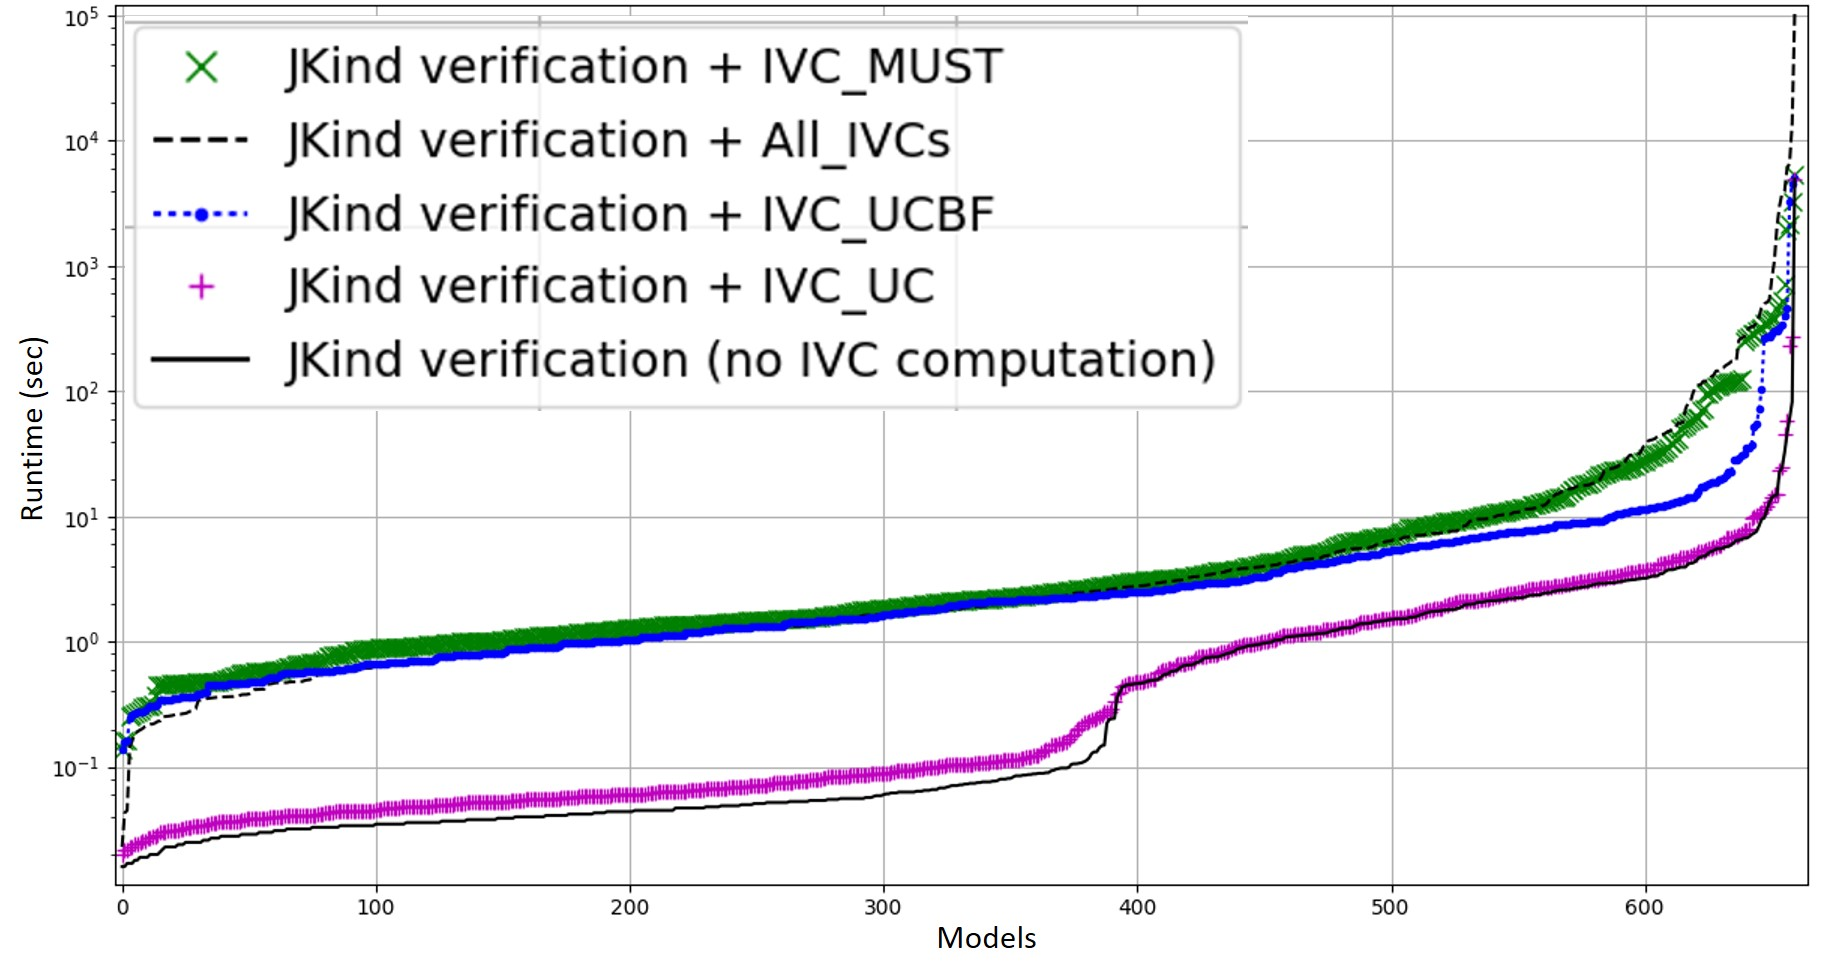
\includegraphics[width=\columnwidth]{figs/timing_cv.jpg}
  %\vspace{-0.2in}
  \caption{Runtime of different analyses}\label{fig:runtimeall}
\end{figure}
\fi

\begin{figure}
  \centering
  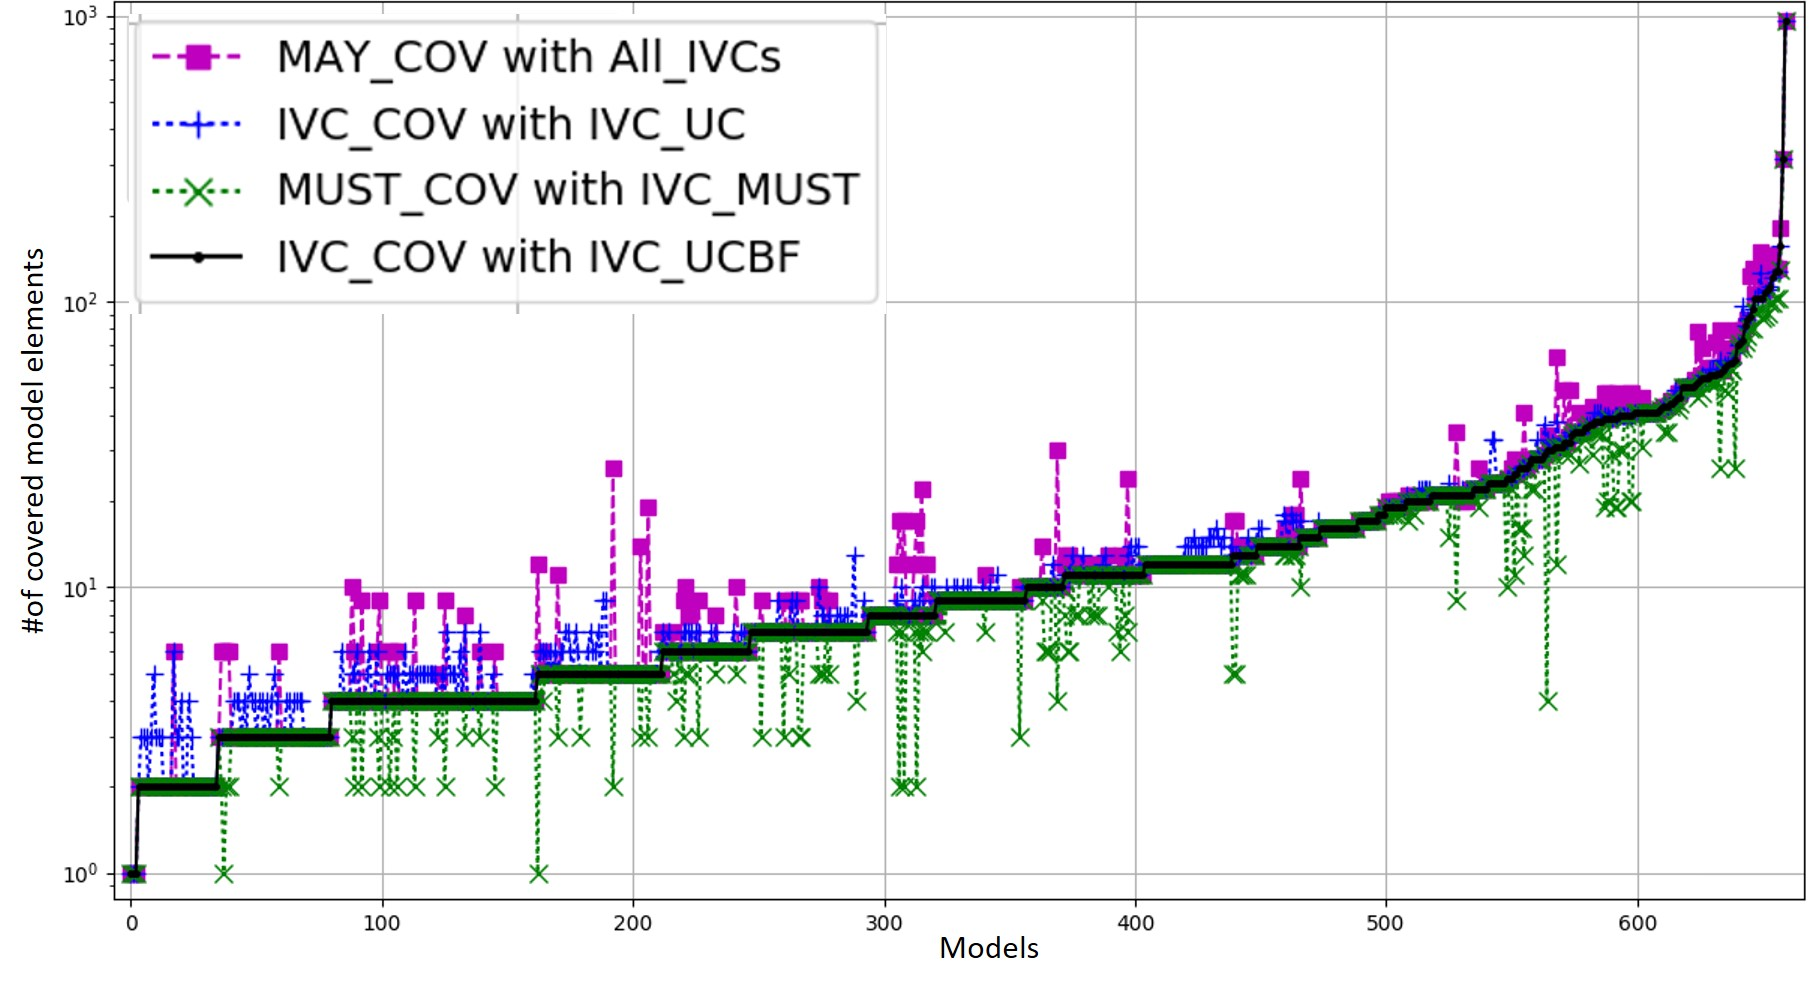
\includegraphics[width=\columnwidth]{figs/cv_size.jpg}
  %\vspace{-0.2in}
  \caption{Size of the set of covered elements by different algorithms}\label{fig:cvsize}
\end{figure}

When a coverage metric brings about lower coverage scores on average,
we say that the metric is harder to satisfy. To study this aspect of the proposed metrics, we first calculated the size of the output sets generated by each algorithm: on average, the ratio of the size of the sets generated by \ucalg\ to the size of the ones obtained from \ucbfalg\ is 1.08,
while this ratio for \mustalg\ to \ucbfalg\ is 0.93, which shows \mustalg\ is harder to satisfy.

Figure \ref{fig:cvsize} is a visualization of the size of the set of covered elements by different algorithms. Models over the x-axis are sorted based on the size of the minimal IVCs obtained from the \ucbfalg\ algorithm.  The graph shows the degree of under-approximation of a minimal proof set by \mustcov\ as well as the degree of over-approximation by \ucalg\ and \maycov.  The proposed coverage metrics can be ranked in terms of their scores as follows:
$$\mustcov \leq \ivccov\ \leq \maycov\ $$
\ivccov\ and \mustcov\ are equivalent when all elements within the model are covered.  If all model elements are part of an \mivc, then there is only one \mivc\ possible and all elements are \must\ elements.

%The equivalence of \mustcov\ and \nondetcovalt\ allows us to compare our algorithms against state-of-the-art mutation based coverage.


%For many analysis problems, this may be accurate enough to

%, which makes \ucalg a reasonable choice for computing \ivccov ~(rather than using \ucbfalg ).
%Therefore, minimality does not dramatically
%affect the coverage scores when \ivccov\ is computed by the \ucalg\ rather than \ucbfalg.
%However, \ucalg might report some elements as covered, while they are not because of the minimality issue.
%And, \mustalg reports some elements uncovered, while they are because it is not able to find \emph{may} elements.

Table~\ref{tab:cov-score} describes the aggregate of the coverage scores returned by the analyses.  Across all benchmarks, the min and max coverage scores are the same, and as expected, the average number of elements required is smallest for the \mustalg\ algorithm and largest the for \ucalg\ algorithm.
One interesting point is that the coverage scores obtained from \maycov\ are not always higher than the scores computed by \ivccov.  Most of the models in our benchmark have only one \mivc. The \ivccov\ score for these models are calculated from the output of the \ucalg\ algorithm, which is not necessarily minimal. However, \maycov\ coverage scores are calculated from the output of \aivcalg\ algorithm, where minimality is guaranteed. Therefore, for the models with \emph{one} \mivc , sometimes \maycov\ yields lower coverage scores as apposed to \ivccov , which balances out the average scores by these metrics (Table \ref{tab:cov-score}).



\begin{table}
  \caption{Coverage scores of different algorithms across all models}
  \centering
  \begin{tabular}{ |c||c|c|c|c| }
    \hline
     score & min & max & mean & stddev \\[0.5ex]
    \hline\hline
    \small{\ivccov}\ with \ucalg &   0.002  & 1.0  & 0.475 & 0.302 \\[0.5ex]
    \small{\ivccov}\ with \ucbfalg&  0.002 & 1.0 &  0.445 & 0.291 \\[0.5ex]
    \mustcov & 0.002 & 1.0 &  0.417 & 0.291 \\[0.5ex]
    \maycov& 0.002 & 1.0 &  0.476 & 0.301 \\[0.5ex]
    \hline
  \end{tabular}
  \label{tab:cov-score}
\end{table}


\iffalse
To investigate the relationship between provability and different coverage notions,
we were interested in the number of models in the benchmark for which
\mustalg\ resulted in the sets not equal to an MIVC (i.e. models for which
\mustalg\ did not preserve provability).
Obviously properties are provable by 100\% of the IVCs computed by \ucalg\ (and \ucbfalg).
As for the \mustalg\ algorithm, the properties of 290 models in the benchmarks were not provable by the output of \mustalg. In practice, for larger models, \mustcov\ is more likely not to maintain provability,
 and since more than half of the models are small, 43\% may still not reveal the actual degree
 to which \mustcov\ underapproximates the covered parts of a model.
  The notion of proof preservation is appealing because it allows a concrete demonstration to the user of the irrelevance of portions of the implementation.  The IVC coverage notion also allows, in cases where there are multiple minimal satisfying sets, insight on multiple ways by which the model meets a requirement.
\fi

%To conclude this section, we should mention that one can define many more proof-based coverage metrics based on the $\mivc$s and $\aivc$s.  Metrics that make use of the $\aivc$ relation are computationally more expensive than \ivccov.


\iffalse
The size of sets computed by \ucalg\ is very close to the size
of the ones obtained from \ucbfalg, especially for larger models.  The average increase in size of IVCs returned by \ucalg\ is approximately 8\% of the \ucbfalg\ algorithm.  Since the overhead of producing \ucalg\ is only approximately 31\% more expensive than the baseline analysis, this test may be efficient enough to run as a standard part of the model checking process.  %If guaranteed minimality is required, the \ucbfalg\ can be used, but
\fi




%\subsection{Optimizing Logic Synthesis}

\input{synthesis}


\section{Discussion}
\label{sec:disc}


\newcommand{\allp}{\texttt{all\_p}}
\newcommand{\onp}{\texttt{on\_p}}
\newcommand{\offp}{\texttt{off\_p}}
\newcommand{\hystp}{\texttt{hyst\_p}}
\newcommand{\aonebelow}{\texttt{a1\_below}}
\newcommand{\atwobelow}{\texttt{a2\_below}}
\newcommand{\aoneabove}{\texttt{a1\_above}}
\newcommand{\atwoabove}{\texttt{a2\_above}}
\newcommand{\doion}{\texttt{doi\_on}}
\newcommand{\done}{\texttt{d1}}
\newcommand{\dtwo}{\texttt{d2}}
\newcommand{\abovehyst}{\texttt{above\_hyst}}
\newcommand{\inhibit}{\texttt{inhibit}}

In this section we show how traceability and coverage analyses can be performed using IVCs.
The goal of this section is to both illustrate the techniques and discuss the potential pitfalls of the analysis. Here we adapt the same ASW example presented in Section \ref{sec:example}. The code is slightly changed so we can discuss how IVCs help to improve the design and specification. 

% \begin{figure}[t]
%\centering
%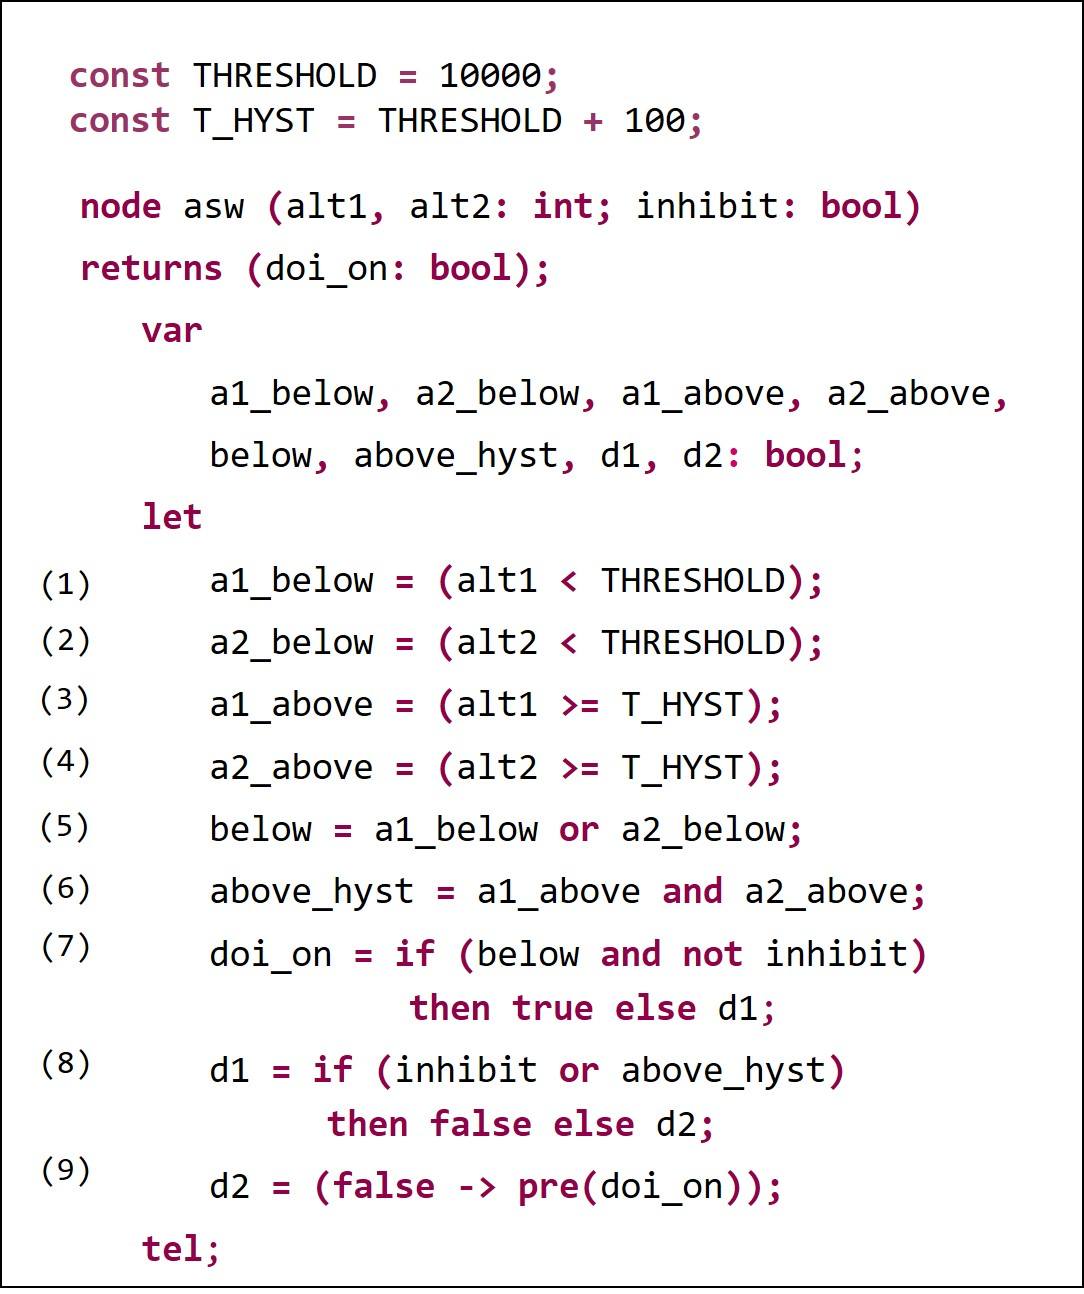
\includegraphics[width=0.9\columnwidth]{figs/code.jpg}
%\vspace{-0.1in}
%\caption{Altitude Switch Model}
%\vspace{-0.1in}
%\label{fig:asw2}
%\end{figure}

 We illustrate the results with traceability matrices produced by the  \texttt{Spear} requirements specification tool~\cite{Spear}.  \texttt{JKind} is used as the model checker for the  \texttt{AADL AGREE} tool suite~\cite{NFM2012:CoGaMiWhLaLu} and also \texttt{Spear} ~\cite{Spear}.  We have extended both tools to add graphical support for displaying adequacy and traceability results.  We show screenshots for the  \texttt{Spear} tool for our running example in Figures~\ref{fig:propertyset1} and~\ref{fig:propertyset4}.

The ASW is responsible for turning on and off a device of interest, so we formulate two requirements that describe when the ASW should be {\em on} and when it should be {\em off}.  The first attempt at formalization (property set 1) is as follows:

%\begin{definition} {\emph{ASW Requirements Version 1} }
{\smaller
\begin{verbatim}
on_p = (a1_below and a2_below) and not inhibit =>
    doi_on = true;
off_p = (a1_above and a2_above) and inhibit =>
    doi_on = false;
all_p = on_p and off_p;
\end{verbatim}
}
%\end{definition}

\begin{figure}
  \centering
  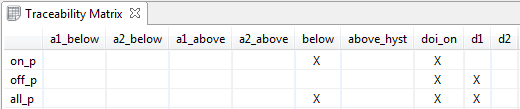
\includegraphics[width=\columnwidth]{figs/spear_set1.png}
  \vspace{-0.1in}
  \caption{Elements covered by the initial property set}
  \vspace{-0.1in}
  \label{fig:propertyset1}
\end{figure}


\noindent Informally, when both altimeters are below the threshold and not inhibited, then the DOI should be on (\onp), and when both altimeters are below the threshold and the ASW is inhibited, then the DOI should be off (\offp).
For each of the \ivccov, \maycov, and \mustcov\ metrics, \allp\ only requires \texttt{\{below, d1, doi\_on\}}, as shown in Figure~\ref{fig:propertyset1}.   This small set of elements is due to a classic specification problem: using computed variables as the antecedents of implications.  If these values are computed incorrectly (say, we choose the wrong threshold for \aonebelow), it may cause the property to be valid for incorrect reasons.

%This is alarming, and somewhat puzzling, because one would think that at least the definitions of the `below' or `above' would be necessary.  However, because the specification used the model variables \aonebelow, \atwobelow, \aoneabove, and \atwoabove, the actual valuations of the thresholds do not matter.  This situation illustrates a classic specification problem: using computed variables in the antecedents of implications.
%\footnote{\noindent ~In this case, if the computation of the variables used in the antecedent is incorrect, then our property will not verify what it is expected to verify \mike{citation to one of our papers on specification here...}; note also that this does not mean the property is necessarily {\em vacuous}.}

We therefore modify our properties to use inputs and constants as antecedents and derive:

{\smaller
\begin{verbatim}
on_p = ((alt1 < THRESHOLD) and (alt2 < THRESHOLD))
   and not inhibit => doi_on = true;
off_p = ((alt1 >= T_HYST) and (alt2 >= T_HYST))
   and inhibit => doi_on = false;
\end{verbatim}
}
% all_p = on_p and off_p;
%\end{definition}

\noindent In this version, distinctions emerge between the metrics.  \allp\ has two \mivc s: \texttt{\{\{a1\_below, below, doi\_on, d1\}, \{a2\_below, below, doi\_on, d1\}\}}, because of the \onp\ property: in the implementation, the DOI is turned on when either of the altimeters is below the threshold, while our property states that they both must be below.
Domain experts determine that the requirement is correctly specified and that our implementation is a reasonable refinement, so there is no need to change the model or the property.  The MUST elements are the same as version 1: \texttt{\{below, doi\_on, d1\}}, because neither \aonebelow\ or \atwobelow\ is required for all proofs.  %However, given the MUST elements, we can no longer construct a proof, because at one of these definitions is necessary for either proof.
The MAY elements contain both \aonebelow\ and \atwobelow.

The \abovehyst, \aoneabove, \atwoabove, and \dtwo\ equations are still missing, meaning that the ``above'' thresholds are irrelevant to our properties.  Examining \offp, we realize that we have a specification error; the DOI should be off if either \inhibit\ is true or both altimeters are above the threshold. The fix is:

%\begin{definition} {\emph{ASW Requirements Version 2} }
{\smaller
\begin{verbatim}
off_p = ((alt1 >= T_HYST) and (alt2 >= T_HYST))
   or inhibit => doi_on = false;
\end{verbatim}
}
%on_p = ((alt1 < THRESHOLD) and (alt2 < THRESHOLD))
%   and not inhibit => doi_on = true;
%all_p = on_p and off_p;
%\end{definition}

\noindent Now the \allp\ requirement proof yields a single \mivc ~that requires all variables except \{\texttt{d2}\}, so \mivc ~= MAY = MUST.  Interestingly, the \offp\ proof requires both the lower altimeter thresholds even though the \onp\ proof does not; the reason is that if either of these is false, then \doion\ will be true.  To cover \{\texttt{d2}\}, we realize no property covers the hysteresis case, so an additional property is added for this case:

%\begin{definition} {\emph{ASW Requirements Version 2} }
{\smaller
\begin{verbatim}
hyst_p = not inhibit and
         (alt1 > THRESHOLD and alt2 > THRESHOLD) and
         (alt1 < T_HYST or alt2 < T_HYST) =>
   (doi_on = false -> doi_on = pre(doi_on))
all_p = on_p and off_p and hyst_p;
\end{verbatim}
}
%on_p = ((alt1 < THRESHOLD) and (alt2 < THRESHOLD))
%   and not inhibit => doi_on = true;
%all_p = on_p and off_p;
%\end{definition}
\noindent The final property states that if the antecedent conditions hold, then in the initial state, the \doion\ variable is assigned false, and in subsequent steps, it retains the same value as it previously had.

\begin{figure}
  \centering
  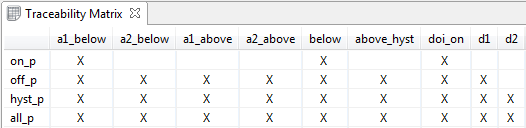
\includegraphics[width=\columnwidth]{figs/spear_set4.png}
  \vspace{-0.1in}
  \caption{Elements covered by the final property set}
  \vspace{-0.1in}
  \label{fig:propertyset4}
\end{figure}

As shown in Figure~\ref{fig:propertyset4}, the measures again coincide and include all variables, and we appear to have a reasonably complete specification.  However, the measures are certainly not foolproof; it turns out that using {\em only} the hysteresis property \hystp\ will {\em also} yield a ``complete'' result for all of the metrics: to establish its validity, all of the equations that we have defined in the model are required.  This is because the partitioning of the transition system (i.e., the equations) is insufficiently {\em granular} to detect the incompleteness.
%However, this one property would not reasonably be considered a complete specification.
Now we will examine this situation.
%We will examine this situation further in the discussion section~\mike{add this!}.
%
%\mike{How would we define a metric that would flag the model as incomplete?  Model transformation would do it: if we added separate variables for each assignment of doi\_on, then any of the metrics would flag the \hystp\ spec as incomplete.}

\iffalse As mentioned, IVCs are derived from inductive invariants; in other words, they are built upon the proof of the validity of a given property. One interesting fact about proofs
  is that a given property could be proved from different proof paths.
  The $AIVC$ captures this fact and gives a clear picture of various ways a property is satisfied. By getting all the MIVCs for the system properties and categorizing them, one can find if there are design artifacts that do not trace to any property: set $\bigcap \{IRR (P) | P \in \Delta \}$.  If this set is non-empty, it is a possible indication of ``gold plating" or missing properties \cite{Murugesan16:renext}.
\fi
%  That is to say, it helps to assess if the specification describe all the behaviors of the system. Being able to measure the coverage of properties over the model is crucial in the safety critical system domain.
Since some of the proposed metrics need to compute all IVCs ($AIVC(P)$),
we have investigated efficient algorithms for computing all IVCs.
Based on our preliminary evaluation, computing $AIVC$ is computationally feasible for realistic models. In addition, we believe that it is possible to obtain MIVCs directly while computing $AIVC$.
We have implemented an efficient algorithm for this purpose, not yet published though. Once the author names are revealed, we can provide a detailed report about it.
%which would remove any concern about minimality. %\ela{this is also mentioned in the RE paper. I don't know if it would be problematic for double-blind reviewing}

\subsection{Granularity}

As we described in Section \ref{sec:background}, transition relation is considered
as the conjunction of Boolean formulas. The granularity of these formulas substantially affects the analysis results.  In the presented example, it was possible to have a ``complete'' specification of the model involving only the hysteresis property \hystp.  The way that the model was structured, in order to determine the validity of the property, all of the equations in the model were required.  However, for this property certain subexpressions of the equations were irrelevant, notably the value assigned to the \texttt{doi\_on} variable in the \texttt{then} branches of equations (7) and (8).  If we decompose the equations into smaller pieces, e.g., creating separate equations for the \texttt{then} and \texttt{else} branches, this incompleteness becomes visible and the model is no longer completely covered.

%Splitting a model into more conjuncts will make coverage scores more accurate and usually lower, though it will not always lower coverage scores.
%
We have recently implemented a transformation that splits models into {\em sufficiently granular} conjuncts such that further decomposition will not cause a complete specification to become incomplete.  We will document this transformation and provide a proof of completeness-result-preservation in future work.
%
In a small initial experiment involving 30 of the original models, we performed our transformation and re-ran the analysis.  By changing the granularity of the model, the analysis tools perform significantly slower for proofs, but the ratio of performance between the proof and the \ucalg\ and \mustalg\ algorithms is largely unchanged.  However, on some models, the \mustalg\ algorithm becomes unacceptably slow (analysis times of 10s of hours) and occasionally causes the solver to run out of memory.

The issue of granularity of models is significant, but tends not to be discussed in detail in previous work.  This will be a focus of our future work, especially in analyzing situations in which the tool determines that a set of requirements is {\em complete}.

%\subsection{Use in Certification}
%Airborne software must undergo a rigorous software development process to ensure its airworthiness. This process is governed by DO-178C: Software Considerations in Airborne Systems and Equipment Certification \cite{DO178C} and when formal methods tools are used, DO-333: Formal Methods Supplement to DO-178C and DO-278A \cite{DO333}. DO-178C proposes a rigorous software development process that starts with an abstract requirements artifact that is iteratively refined into a software designs, source code, and finally, object code, and a set of {\em objectives} that should be met by critical avionics software.  Two of the key tenets of this process are traceability and adequacy; that is, each refinement of an artifact must be traceable to the artifact if was derived from. Further, each refinement must be shown not to introduce functionality not present in the artifact from which it was derived (adequacy). For example, DO-178C objectives A-3.6 (traceability of high-level requirements to system requirements) and A-4.6 (traceability of software design to high-level requirements) specifically require applicants to demonstrate bi-directional traceability.
%
%DO178C currently uses a variety of metrics to determine adequacy of requirements, but much of the effort involves code-level testing.  Test suites are derived from requirements and used to test the software and measured using different structural coverage test metrics.  If code-level test suites do not achieve full coverage, then an analysis is performed to determine whether there are missing requirements and test cases.  The kind of structural coverage required (e.g., statement, branch, MCDC) for adequate testing is driven by the criticality of the software in question.
%
%The utility of the proposed metrics are being evaluated by Rockwell Collins on a pilot project. The proposed metrics
%appear to be useful for both traceability and adequacy checking \cite{lucas17}.  The proposed metrics appear to be useful for both traceability and adequacy.  Previously, bi-directional traceability between artifacts involved rigorous manual peer review to determine that requirements were adequate and that additional functionality was not introduced in the implementation model.  In the pilot approach, both traceability and adequacy are assessed using metrics proposed in this paper.  The goal is to use this automation to satisfy the DO178C objectives related to traceability and adequacy.


%We plan to focus on efficient analysis of sufficiently granular models in future work.
%when the tool returns that the set of requirements are complete.






\section{Conclusions \& Future Work}
\label{sec:conc}
The idea of extracting a minimal IVC for a given property, and applications for doing so was recently introduced in \cite{Ghass16}.  However, a single IVC often does not provide a complete picture of the traceability from a property to a model.  In this paper,
we have addressed the problem of extracting {\em all minimal} IVCs. We have shown
the correctness and completeness of our method and algorithm.  In addition, we have a substantial evaluation that shows that the practicality and efficiency of our technique.

Our method is inspired by a recent work in the domain of satisfiability analysis \cite{marco2016fast}. One interesting future direction is to devise similar MIVC enumeration algorithms based on other studies on MUSes extraction such as \cite{nadel2014accelerated}.  We are also looking into improving our implementation by using more  efficient methods for the \isadeq ~and \getivc ~modules used by our algorithm. Another interesting direction is to parallelize the enumeration process: it is certainly possible to ask for multiple distinct maximal models to be solved in parallel.
%, though this may result in unnecessary work performed by some of the parallel solvers.

We also plan to investigate additional applications of the idea.  When performing {\em compositional verification}, the All-IVCs technique may be able to determine {\em minimal component sets} within an architecture that can satisfy a given set of requirements, which may be helpful for design-space exploration and synthesis. Finally, we are interested in adapting the notion of (all) validity cores for \emph{bounded} model checking for quantifying how much of models have been explored by bounded analysis. 
% % \input{RelatedWork}
% % \input{ModelDevelopment}
% % \input{Discussion}
%\chapter{Conclusions}
  
In this proposal, we introduce the idea of extracting a minimal IVC for a given property and its applications.  However, a single IVC often does not provide a complete picture of the traceability from a property to a model.  We would also like to address the problem of extracting {\em all minimal} IVCs. 
We will show
the correctness and completeness of our methods and algorithms.  In addition, we plan to have a substantial evaluation that shows that the practicality and efficiency of our technique. For this purpose, we have collected a large set of benchmarks from different sources. Our experiments are conducted on a set of benchmarks containing 660 Lustre models, 530 from~\cite{Hagen08:FMCAD, piskac2016} and 130 industrial models derived from \cite{hilt2013} and other sources \cite{piskac2016, NFM2015:backes}.  Most of the academic benchmark models are small (10kB or less, with 6-40 equations) and include a range of hardware benchmarks and software problems involving counters that are difficult to solve inductively.
The industrial models are much larger; for example, each 80 models from \cite{hilt2013} contain over 600 equations and are each $\geq$80kB in size. The benchmark includes 2 models from NASA Quad-redundant Flight Control System (QFCS)~\cite{NFM2015:backes}: the Flight Control System (FCS) with 5259 Lustre equations and the Flight Control Computer (FCC) with 10969 equations.

We selected only benchmark problems consisting of a Lustre model with
properties that JKind could prove with a 3-hour timeout.
Experiments are run in a configuration with the \texttt{Z3} solver and the ``fastest'' mode of JKind (which involves running the $k$-induction and PDR engines in parallel and terminating when a solution is found). The experiments are expected to be run on an  Intel(R) i5-4690, 3.50GHz, 16 GB memory machine running Linux, and available online.

Our method for computing all MIVCs is inspired by a recent work in the domain of satisfiability analysis \cite{marco2016fast}. One interesting future direction is to devise similar MIVC enumeration algorithms based on other studies on MUSes extraction such as \cite{nadel2014accelerated}. 
Another interesting direction for this project is to parallelize the enumeration process: it is certainly possible to ask for multiple distinct maximal models to be solved in parallel.
%, though this may result in unnecessary work performed by some of the parallel solvers.

We also plan to investigate additional applications of the idea.  When performing {\em compositional verification}, the All-IVCs technique may be able to determine {\em minimal component sets} within an architecture that can satisfy a given set of requirements, which may be helpful for design-space exploration and synthesis. Finally, we are interested in adapting the notion of (all) validity cores for \emph{bounded} model checking for quantifying how much of models have been explored by bounded analysis.

Upon completion of the proposed research, we will have our IVCs computation algorithms integrated in the JKind model checker. The implementation will be benchmarked and evaluated rigorously. The usefulness of the IVC idea will be shown by utilizing its applications into different projects.


% \printglossary[title={LIST OF TERMS}, toctitle={List of Terms}]

%%%%%%%%%%%%%%%%%%%%%%%%%%%%%%%%%%%%%%%%%%%%%%%%%%%%%%%%%%%%%%%%%%%%%%%%%%%%%%%%
% WORKS CITED
%%%%%%%%%%%%%%%%%%%%%%%%%%%%%%%%%%%%%%%%%%%%%%%%%%%%%%%%%%%%%%%%%%%%%%%%%%%%%%%%
% When you need a works cited section, uncomment this and update the name of the
%   file.
%%%
 %   \bibliographystyle{abbrv}

%\bibliography{noAbbreviations,citations}

\putbib
\end{bibunit}
%%%%%%%%%%%%%%%%%%%%%%%%%%%%%%%%%%%%%%%%%%%%%%%%%%%%%%%%%%%%%%%%%%%%%%%%%%%%%%%%
% APPENDICIES
%%%%%%%%%%%%%%%%%%%%%%%%%%%%%%%%%%%%%%%%%%%%%%%%%%%%%%%%%%%%%%%%%%%%%%%%%%%%%%%%
% If you need an appendix, uncomment the following lines and add sections.
%%%
\def\noprint#1{\relax}
\renewcommand\bibname{List of Publications}
\begin{bibunit}
\defaultbibliographystyle{unsrt}
%\bibliography{mypapers}
\noprint{\cite{journal,jk,c0,c1,c2,c3,Mur16}}
%\cite{journal,jk,c0,c1,c2,c3,Mur16, memocode15, multiformalism2014}
%\ifthenelse{\boolean{IncludeVersionHistory}}{
%\unvbox\vhbox
%}{
%\cite{journal}
% \cite{jk}
% \cite{c0,c1,c2,c3}
% \cite{Mur16, memocode15, multiformalism2014}
%\bibname
%}

\putbib
\end{bibunit}
\end{document}
